\documentclass[12pt]{article}
\setlength{\voffset}{-0.4in}
\setlength{\hoffset}{-0.4in}
\addtolength{\textwidth}{0.75in}
\addtolength{\textheight}{0.75in}
\renewcommand{\baselinestretch}{1.0}
\newcommand{\smallcirc}{\mathbin{\text{\raisebox{0.2ex}{\scalebox{0.6}{$\circ$}}}}}
\usepackage{latexsym,amsfonts,epsfig,eucal, amsmath, amssymb,amsthm,tikz,pgfplots,stmaryrd}
\usepackage{enumitem}% http://ctan.org/pkg/enumitem
\usepackage{tikz-cd}
\usepackage{pgfplots}
\pgfplotsset{compat=1.15}
\usepackage{mathrsfs}
\usepackage[style=authoryear,backend=biber,natbib]{biblatex}
\addbibresource{SEURef.bib}
\usetikzlibrary{arrows}
\renewcommand\qedsymbol{$\blacksquare$}
\begin{document}
\title{Expected Utility from a Constructive Viewpoint}
\author{Kislaya Prasad\\University of Maryland\footnote{Address:
    Robert H. Smith School of Business, University of Maryland, College Park, MD
    20742, U.S.A. Telephone: +1 (301) 405-6359. Email: kprasad@umd.edu.}}
\date{February 13, 2023} \maketitle
\begin{abstract}
This paper proves a constructive version of the expected utility theorem. The word ``constructive'' is construed here in two senses---first, as in constructive mathematics, whereby the logic underlying
proofs is intuitionistic. In a second sense of the word, ``constructive'' is taken to mean ``built up from simpler components.'' Preferences are defined over lotteries that vary continuously over some
topological space, and are themselves assumed to vary depending upon some underlying process of measurement, deliberation, or observation. The open sets of the
topology serve as the possible truth values of assertions about preference and constrain what can be measured, deduced, or observed. Replacing an open set by an open covering of smaller sets serves
as a notion of refinement of information, and deductions made for these smaller sets can be combined or collated to yield corresponding deductions over the larger set. The two notions of constructive
end up being related because the underlying logic of the objects so constructed turns out to be intuitionistic. The classical expected utility theorem is shown to be non-constructive, and a constructive version
is proved for the present setting by narrowing the domain of preferences. The representation of preferences is via comparisons of continuous real-valued functions.
A version of the classical theorem is obtained by imposing a restriction on the collection of open sets of the topology, which has the effect of making the logic classical. The proof here illustrates a
robustness property of constructive results---they can be carried over virtually unchanged to a variety of mathematical settings. Here the set of variable lotteries replaces the sets of lotteries from the
classical setting, but there are other possibilities.

\bigskip

\noindent {\bf JEL classification:\/} C72, C79, C91.

\smallskip

\noindent {\bf Keywords:\/} Expected utility theorem, constructive, intuitionistic logic, sheaf theory.
\end{abstract}
\newpage
\section{Introduction}
This paper proves a constructive version of the expected utility theorem. The word ``constructive'' is construed here in two senses---first, as in constructive mathematics,
whereby the logic underlying proofs follow intuitionistic logic. Intuitionistic proofs eschew use of the law of the excluded middle and proofs by contradiction on the grounds that objects
proved to exist using such rules may not be computable or algorithmically realizable. In a second sense of the word, ``constructive'' is taken to mean ``built up from simpler
components.'' The decision-maker is not assumed to have pre-existing, well-defined, preferences that need only to be interrogated. Instead, they are defined over lotteries that vary
continuously over some topological space, and are also assumed to vary with the state of knowledge of the decision-maker. This knowledge depends upon some underlying process
of measurement, deliberation, or observation. We abstract from the details of this process. However, some such process of variation is necessitated by
the requirement that preferences must be allowed to be different based on different outcomes of measurement, deliberation, or observation.
The open sets of the topology serve as the possible truth values of assertions about preference and constrain what can be measured,
deduced, or observed. Replacing an open set by an open covering of smaller sets serves as a notion of refinement of information, and deductions made for these smaller sets
can be combined or collated to yield corresponding deductions over the larger set (this is our second notion of constructive at work). Mathematically, the structure which
serves as the setting for this paper is a sheaf on a topological space. The two notions of constructive end up being related because the underlying logic of sheaves is in general
intuitionistic. With variable lotteries, the classical expected utility theorem is shown to be non-constructive, and a constructive version is proved for the present setting by
narrowing the domain of preferences. The representation of preferences is via comparisons of continuous real-valued functions. A version of the classical theorem is obtained
by imposing a restriction on the collection of open sets of the topology, which has the effect of making the logic classical. The proof here illustrates a robustness property of
constructive results---they can be carried over virtually unchanged to a variety of mathematical settings. Here the set of variable lotteries replaces the sets of lotteries from the
classical setting, but there are other possibilities discussed in the conclusion of the paper.

In the framework introduced here, lotteries vary continuously over a topological space $X$ (i.e., are continuous functions from $X$ to the space of lotteries).
Preferences are defined directly over these functions, as well as over restrictions of the functions to open subsets of $X$. Preferences may also vary over $X$.
The collection of open sets of $X$, denoted $\mathcal{O}(X)$, plays an important role here as the set of possible {\em truth values\/} for questions such as
``When is the variable lottery $f$ preferred to variable lottery $g$?'' or ``When is the decision-maker indifferent between variable lotteries $f$ and $g$?''
The classical setting is a special case of this framework where $X$ is the singleton space with open sets $X = \{*\}$ and $\emptyset$. So, classically, the only
possible answers to the above questions are $X$ (``always") or $\emptyset$ (``never"). However, when lotteries and preferences vary over more general spaces,
the answer may be only some part of $X$. The topology places restrictions on what the possible answers to the above questions can be. If $\mathcal{O}(X)$
consists of {\em all\/} subsets of $X$, then the requirement that possible answers be open sets is not restrictive. However, for other topologies the requirement
can be genuinely restrictive, and involves choosing the largest open set for which the asserted ranking holds. A slightly different way of stating this is that, at any
$x\in X$, the decision-maker can assert some ranking of a pair of variable lotteries if and only if the same ranking holds at all $y$ in some open neighborhood $U$ of $x$.

An immediate consequence of the manner in which assertions of preference are made above is that, unlike in the classical setting,
there will be points in $X$ at which two variable lotteries are not comparable. The following example illustrates this -- suppose there are two variable lotteries $f$ and $g$
and a point $x$ such that every open neighborhood $U$ of $x$ contains two open subsets $V_1$ and $V_2$ with $f$ preferred to $g$ for all $y\in V_1$ and $g$
preferred to $f$ for all $y\in V_2$. Then there can be no neighborhood of $x$ in which either one of $f$ or $g$ is preferred to the other, making them uncomparable.

In the case of variable lotteries, a distinction exists between indifference and non-comparability.
Indifference can be defined in the usual way for a pair of variable lotteries as
the assertion that neither of the two is better than the other. However, the appropriate definition of negation in the current framework is as follows---for some proposition $P$,
we assert $\neg P$ over $U\in \mathcal{O}(X)$ if and only if $P$ does not hold for any open $V\subseteq U$. In the case of two lotteries $f$ and $g$, indifference over $U$
requires that for no $V \subseteq U$ can we assert that either of $f$ or $g$ is better than the other (when $f$ and $g$ are restricted to $V$). So, there are three possibilities:
the decision-maker (1)~is indifferent between $f$ and $g$, (2)~prefers one of $f$ or $g$ to the other, and (3)~is unable to compare $f$ and $g$. Since (1) and (2) are
negations of one another, we have a violation of the law of the excluded middle, the principle of classical logic asserting that either a proposition is true or its negation is true. This
will be seen to have significant implications for the development of our theory.

There is another way to reason about ranking lotteries which begins with the assertion of an open set $U\subseteq X$ and asks what rankings then hold? For instance, if the
truth value of ``$f$ is preferred to $g$'' contains $U$, then the assertion of $U$ allows us to assert ``$f$ is preferred to $g$''.
Assertions of open sets will correspond, in this framework, to observations, measurements, computations or deductions about the point $x$ in $X$ that obtains
(i.e., the assertion of $U$ is the confirmation that $x\in U$). Only the opens $U$ to which $x$ belongs can be known, with the point $x$ being unknown
(unless $\{x\}$ is itself open). Few restrictions are placed on either the space $X$ or the topology $\mathcal{O}(X)$. $X$ can be time, locations in space, stages of
accumulated knowledge, and so on. The points of $X$ will be referred to as {\em stages\/} (to distinguish them from {\em states\/}, which already have established
usage in expected utility theory). The collection of open sets are potential observations, computations, measurements, or deductions about the point in $X$ that holds.
As will be shown later in the paper, the collection of open sets respects the logic of finite observation and finitely terminating computations.
This is a consequence of the definition of a topology in that the arbitrary conjunction (union) and finite disjunction (intersection) of open sets will still be open.
However, the complement of an open set need not be open. The topological model of information presented here will be seen, in Section~2, to extract the essential
features of the accumulation of knowledge
and of many different ways of obtaining information. In this instance, the information is used to determine the ranking of lotteries, but many other applications
of the idea are possible. One can choose $\mathcal{O}(X)$ to impose bounds on the decision-maker's ability to identify the stage exactly, and the
special case where there is no such bound will be seen to correspond to the classical case. Continuity also plays an important role here, capturing essential
computational and observational notions. The continuity of variable lotteries ensures that observational constraints built into the topology are not violated.
One cannot, from measurements of the outcome, make any deductions or assertions about the stage that would not be possible using just the open sets.

An appealing feature of the present approach is that it provides a natural way of thinking about refinement of information and of obtaining better approximations
of preference rankings. If we think of an open set $U$ as carrying information about the value of $x\in X$ that obtains, then
a smaller open set ($V \subset U$) provides more refined information. It is an assumption of the theory that if $U$ allows us to assert ``$f$ is preferred to $g$'', then this
ranking should continue to hold when we assert some $V \subset U$ (i.e., an assertion of preference, once made, cannot be retracted when more detailed information
becomes available). With this assumption, refinement reveals new rankings, as variable lotteries that were previously not comparable become comparable.

The intent here is to represent preferences using a continuous real-valued expected utility function defined over $X$. The expected utility function is defined
pointwise as the probability weighted average of a utility of consequences or prizes. The lottery is continuous over $X$ by assumption, and the utility
needs to be proven to be continuous. Real-valued functions $r, s: X\rightarrow \mathbb{R}$ are ordered in the same way that lotteries are ranked: at some $x\in X$
$r<s$ if and only if there is an open neighborhood $U$ of $x$ such that for all $y\in U$ $r(y)<s(y)$ (equivalently, the truth value of $r<s$ is the largest open set
over which $r<s$). So, if upon assertion of an open set $U$ we are able to assert ``$f$ is preferred to $g$'' then we are also able to assert that the expected utility
of $f$ is greater than the expected utility of $g$. Similarly, indifference between $f$ and $g$ entails equality of their expected utilities.
However, if $f$ and $g$ are not comparable over $U$ in terms of preference,
then the expected utilities of $f$ and $g$ are not comparable in terms of $<$ over $U$ either.
Refinement of information typically leads to a ranking of previously uncomparable
variable lotteries and, correspondingly, new rankings in terms of expected utility. However, it is possible that in some stages there are lotteries that can never be
compared.

The approach to the proof here is closely tied to the idea of ``constructive'' proofs in mathematics. There is a long tradition in mathematics which
insists that objects proved to exist should be algorithmically realizable or computable \citep[see][]{bridgesrichman1987}.\footnote{Section~2 of this paper
also provides a brief survey.}
This tradition rejects use of the law of the excluded middle, which is the principle of classical logic stating that for every proposition $P$, either $P$ is true or its
negation $\neg P$ is true. Also rejected is proof by contradiction (for every $P$, $\neg\neg P \Rightarrow P$), which is an implication of the law of the
excluded middle. These logical rules are the culprits
behind the fact that using classical logic it is possible to prove existence of objects that are not algorithmically realizable.
The logical system used in constructive mathematics, distinguished principally by the omission of the law of the excluded middle, goes under the
name of intuitionistic logic. The current paper
is not concerned with the philosophical debates about how mathematics ought to be conducted. However, a very practical issue arises in the framework outlined
above---the law of the excluded middle does not hold. There was an intimation of this in the demonstration above that comparisons of a pair of lotteries lead to
three distinct possibilities: (1) one lottery is judged to be better than the other, (2) the decision-maker arrives at the conclusion that she is indifferent between the two, or
(3) she is unable to make a comparison. For this reason, we use only constructive arguments when proving results.

The idea for the proof is to leave the expected utility theorem unchanged (i.e., in the way it is stated in the familiar universe of set theory), and change the
universe itself to a ``generalized'' universe of sets ({\em viz.\/}, a universe of variable sets). To elaborate on what this sentence means, we begin
with the observation that the set of variable lotteries described above is a mathematical object called a sheaf \citep[see][]{maclane1996}.
The set of all continuous real-valued functions defined over $X$ is also a sheaf. Now the category of sheaves on a topological space $X$ may be
thought of as a generalized universe of sets where all sets are varying continuously over $X$
(i.e., a universe of ``variable sets'').\footnote{\citet{maclane1996} develop the idea of a topos as a generalized universe of sets. The universe of sheaves is a
topos, and can be interpreted as a universe of variable sets. One can specialize to the familar universe of sets by taking $X$ to be the singleton space, or by
making all objects constant.} Within this mathematical universe, which will be denoted as Sh($X$), one can carry out familiar set-theoretic
constructions. For instance, one such construction is of the real numbers as a Dedekind cut of the rational numbers. This construction leads to the real numbers in
Sh($X$) being (isomorphic to) the sheaf of continuous real-valued functions over $X$. Sh($X$) has an internal language within which one can state formulae or
sentences, just like in the familiar universe of sets. The important difference between the two is
that the rules of inference for Sh($X$) are the rules for the first order {\em intuitionistic\/} predicate calculus. This system of logic is like classical logic, except that
the law of the excluded middle is absent. A consequence is that theorems with constructive proofs can be carried over to the universe of sheaves, whereas classical
results carry over only to some special cases (such as the singleton space discussed earlier). Given the ``constructive flavor'' of the expected utility theorem,\footnote{Evident
in the proof, but even more so in expositions such as \citet{pratt1964}. }
and the fact that the set of variable lotteries and the set of all continuous real-valued functions are sheaves, it is a reasonable conjecture that one can state and prove
the expected utility theorem for Sh($X$). One would define suitable preference orderings over the variable lotteries, and
find an order-preserving mapping from variable lotteries to the continuous real-valued functions. Since we are keeping the expected utility theorem unchanged,
we attempt to prove this result using only the axioms in classical expected utility theory. These are the weak order,
independence, and continuity assumptions. Developing a theory based on rankings of functions and their restrictions to open sets, raises a number of challenges. As shown
later in the paper, important properties of preferences, such as negative transitivity, appear not to carry over when functions (or their parts) are ranked. However, we are
able to state versions of the same axioms for functions that can be used to prove the results. Additionally, in Sh($X$) the Dedekind reals are not equivalent to the
Cauchy reals, and the former is the appropriate construction that yields the desired representation result.

We turn now to the results that are actually proved.
Unfortunately, the expected utility theorem turns out to be non-constructive. This is shown in Example 2, where we present a topology and define preferences such that
representation using a continuous real-valued expected utility function is not possible. The difficulty here relates to stages in $X$ where no two lotteries are
comparable. In the classical setting, if no two lotteries can be ranked we are able to infer indifference between every pair of lotteries (by an application of the law of
the excluded middle). Clearly, this cannot be done in the constructive setting. One approach for obtaining the intended representation of preferences is to narrow down
the class of preferences. This is done via an additional assumption called minimal comparability---on {\em a priori\/} grounds, one is able to assert that either (1)~there exist
two lotteries $f$ and $g$ such that one is preferred to the other, or (2)~the decision-maker is indifferent between all lotteries. Together with the standard assumptions, this
condition is sufficient to ensure representation of preferences via a continuous real-valued expected utility function. This result is Theorem~1 of the paper.
However, the necessity part of the classical expected utility theorem no longer holds. The minimal comparability requirement
is {\em local\/} in the sense that one of the above conditions is known to hold in an open neighborhood of every point $x\in X$.
However, it could be that the condition~(1) above is satisfied by a different pair of lotteries in different
parts of $X$. Then we would have an expected utility for every lottery in an open neighborhood of each stage in $X$, but it may not be possible to ``glue'' them together
into a global function over all of $X$. We need a slightly stronger version of the minimal comparability condition to ensure a representation using a {\em global\/} utility
function. This result is proved in Corollary~1. In Theorem~1 and Corollary~1, both
lotteries and preferences are allowed to vary. For Corollary~2, we impose the requirement that rankings of constant lotteries never change over $X$---i.e., for any pair of constant lotteries
$f$ and $g$, either $f$ is preferred to $g$ over all of $X$ or $f$ is never preferred to $g$ (and similarly for $f$ indifferent to $g$ and $g$ is preferred to $f$). This assumption
has the effect of arresting the variation in the utility function so that the utility of any consequence or prize (i.e., the utility of the degenerate distribution on the prize) becomes constant
over $X$. The expected utility function is still variable, but all the variation comes from the variation in lotteries.

The second approach to obtaining a representation result is by assuming that the sheaf satisfies the law of the excluded middle---for all propositions $P$ either $P$ or $\neg P$. An equivalent formulation of this classical logic assumption is the following requirement for the topology $\mathcal{O}(X)$:
for every open set $W$ in $\mathcal{O}(X)$ we have $W \cup \mbox{Int}(W^c) = X$, where $\mbox{Int}(W^c)$ is the interior of the
complement of $W$. This law is, of course, implicitly assumed in the classical expected utility theorem. We present a version of the classical result for the framework in Theorem~2. Together with the weak order, independence, and continuity axioms, the classical logic assumption provides necessary and sufficient conditions for the representation of preferences using a continuous real-valued expected utility function. As might be expected, the phenomenon of non-comparability now disappears.

{\it Related Literature.\/} The word ``constructive'' has been used in a different sense in the recent decision theory literature, but the goals are related. A central idea is to begin with a decision problem confronting a decision-maker and then to characterize the process by which value judgments and probability assessments are formed to guide choices. In this vein, \citet{blume2021} begin with a natural language description of a decision problem and derive states, outcomes, and Savage acts, and from this derive an expected utility representation. \citet{shafer2016} makes the point that a fully constructive theory should include an account of how probability and value judgments are formed, and then inform preferences. In particular, in his view, preferences should follow probabilities and utilities instead of the latter being elicited from preference. He is sceptical of the ability of expected utility to provide such a constructive theory, and presents an alternative. Perhaps the closest to the present paper is that of \citet{kaneko2020}, who models a form of bounded rationality in which permissible probabilities are restricted to decimal fractions of finite depth up to a given bound. This leads to the phenomenon of non-comparability, with the problem being worse when
the cognitive bound is smaller. He obtains a representation in terms of a two-dimensional vector-valued utility function with the interval order. The expected utility hypothesis holds in his framework when the bound goes to infinity. The sense in which the term ``constructive'' is used in the present paper is taken from constructive mathematics. In this sense of the word, the constructive development of preference and utility was pioneered by Douglas Bridges \citep{bridges1982, bridges1989,bridges1994}) within the constructive framework of Errett Bishop \citep{bishop1967}. This is a framework that does not allow use of the law of the excluded middle). \citet{richter1999} present a development within computability theory. The present paper focuses on choice under uncertainty and models preference and expected utility in a setting with variable lotteries, with a topology being used to encode essential observational or computational restrictions (in other words, within the category of sheaves). The extensive literature upon which our theory is built is discussed in Section~2 of the paper. The law of the excluded middle need not hold, the proof needs to be constructive in this second sense. However, this paper's point of view is intermediate to these two approaches. The decision maker is viewed as making assertions about the world (the open sets) that entail assertions of preference between variable lotteries. These assertions are presumed to derive from some evaluation of evidence. We have abstracted from what this evidence is about, but the requirement of a topology enforces a logic of evidence for these assertions, and the representation respects the same logic.

The following is an outline of the remainder of the paper. We begin in Section~2 with a short survey of key ideas in constructive mathematics and sheaf theory. The objective is make the paper relatively self-contained. We also present a number of examples of phenomena of measurement, computation, and observation and illustrate how an intuitionistic logic applies, and how these can be put into a common topological setting. Section~3 contains the main results paper, including the constructive expected utility theorem for variable lotteries, and its specialization when classical logic applies. Section~4 contains concluding remarks. The proofs are in the appendix which follows the references.

\section{Brief Survey of Constructive Mathematics and Sheaves}
The purpose of this section is to make this paper relatively self-contained. To this end, we provide an introduction to ideas in constructive mathematics and in sheaf theory. Additionally, we elaborate on the link between topology and computation, which plays a central role in this paper. The topics and emphasis are chosen to ease exposition of the results in this paper, and the tone is informal with the focus being on providing the intuition behind key results. More formal and complete surveys of the subject can be found in the various references cited in this section. \citet{bauer2017} is a good short introduction, while \citet{goldblatt1982}, \citet{bridgesrichman1987}, \citet{maclane1996}, and \citet{vickers1996} provide more comprehensive surveys.
In this section, we begin by describing what constructive mathematics is. This is followed by a comparison of classical and intuitionistic logic. Following this are examples
of phenomena for which the appropriate logic is intuitionistic, We then discuss sheaves and their properties, emphasizing their nature as a universe of variable sets. Finally, we show how mathematical statements can be stated within this universe, and how the truth of these statements are deduced.

Constructive mathematics is done without the {\it law of the excluded middle\/}: this principle of logic states that for every proposition
$p$, either $p$ is true or its negation $\neg p$ is true ($\forall p, p\vee \neg p$). A consequence of the law is that proof by contradiction is unacceptable. Such a proof rests on the notion that if a proposition can be shown to be not false, then one can conclude it is true ($\neg \neg p \Rightarrow p$). Also unacceptable is the axiom of choice, which has been shown to  imply the law of the excluded middle \citep[see][ p.~483]{bauer2017}.
The name ``constructive mathematics" derives from the fact that objects proved to exist by constructive methods
are {\it algorithmically realizable\/} or {\it computable\/}. In other words, if something is asserted to be true, there is an algorithm witnessing its truth, and if something is asserted to exist, it is possible to construct it through an explicit computation. A non-constructive proof can sometimes, but not always, be replaced by a constructive proof. However, there are instances where there can be no algorithm to construct an object purported to exist. In such instances, the culprit has been found to be the law of the excluded middle.

An oft-cited example of a proposition that can be asserted in classical mathematics, but not in constructive mathematics, is the assertion that every real number is either equal to zero or different from zero: $(\forall x \in \mathbb{R}) (x = 0 \vee x \neq 0)$. This classically valid assertion -- true by the law of the excluded middle -- is considered constructively suspect. There can be no general method for determining, for an arbitrary real number $x$, if $x=0$ or $x \neq 0$. To see why, consider the still unsolved Goldbach conjecture, which states that every even natural number greater than $2$ is the sum of two prime numbers \citep[see][p.~98]{bridges1999}.
Consider the ordered sequence of even natural numbers greater than $2$ ($\{4, 6, 8, \ldots \}$) and construct
the sequence $\{\alpha_k\}$ as follows. For each member of the former sequence it is possible to determine finitely whether it is the sum of two prime numbers or not. If the $k$-th member of the sequence is the sum of two primes, set $\alpha_k =0$; if not, set $\alpha_k =2^{-k}$. Define $\alpha = \sum_{k=1}^\infty \alpha_k$. So we have constructed a real number $\alpha$ such that the Goldbach conjecture is true if and only if $\alpha =0$. If the conjecture fails,
then $\alpha > 0$. Note that $\alpha$ is a real number because $\sum_{k=1}^n \alpha_k$ provides us with a convergent sequence of rational numbers,
yielding as close an approximation to $\alpha$ as we want (for $n$ large enough). Any general method for determining whether an
arbitrary real number is equal to zero or different from zero could be used to resolve the Goldbach conjecture.\footnote{There are other versions of this
result. For instance, \citet{turing1936}, p.~248, states a similar result about his ``computable'' real numbers.}
It is worth noting that the Goldbach conjecture has been confirmed for integers less that $4 \times 10^{18}$.\footnote{See the Wikipedia entry on Goldbach's conjecture.}
By checking specific instances one can never hope to affirm the conjecture, however it is possible to refute it by finding a specific instance of failure.
The observation content of a proposition and its negation can be quite different.
Examples such as the above, which show that solutions for certain problems would imply solutions for other problems for
which no solutions are known, go under the
name of ``Brouwerian counterexamples."

Constructivists such as Brouwer also questioned the meaning of existence in circumstances where the object claimed to exists was not algorithmically realizable.
They would deny that to assert existence it is sufficient to show that the assumption that the object does not exist creates a contradiction.
A number of familiar results in mathematics (the intermediate value theorem, the extreme value theorem, etc.) turn out not to be constructively valid in this sense.
Take the example of the extreme value theorem. Here, we use a closely-related fact to the previous example: one cannot in general decide, for
arbitrary real number $x$, whether $x\geq 0$ or $x\leq 0$ \citep[see][p.~100]{bridges1999}.
Assume that $f$ is a continuous function on $[0,1]$. The function is assumed to be
computable in the sense that one can obtain arbitrarily close approximate to $f(x)$ by taking suitably close approximations of the argument $x$.
It turns out that one cannot always approximate a point $x^*$ for which the function attains its maximum.The reason is related to the fact that the
{\em argmax\/} of $f$ can be discontinuous, and around the points of discontinuity the potential maximum points can be far apart.
Consider for instance $f$ defined on $[0, 1]$ by $f(x) = (1+\alpha) x + (1-\alpha) (1-x)$. Here, $\alpha$ is a real-valued parameter which
can be approximated arbitrarily closely. As a result, approximations to $x$ can be translated into those of the value of $f$.
Now, if $\alpha > 0$, then $x^*=1$. If $\alpha <0$, then $x^*=0$.  If $\alpha = 0$, then any $x^*\in [0,1]$ is a maximum point.
An algorithm to compute approximations of $x^*$ would enable us to determine for arbitrary $\alpha$ if $\alpha \geq 0$ (when $x^*$ is
in the neighborhood of 1 that excludes 0) or if $\alpha \leq 0$ (when $x^*$ is in the neighborhood of 0 that excludes 1).
If this were true for arbitrary $\alpha$, we would have a general method for determining for an arbitrary real number $x$, whether
$x\geq 0$ or $x \leq 0$. .
In contrast to the maximum point, the maximum {\it value\/} of $f$ can be computed (e.g., by taking the maximum value
over a suitably fine grid of points of $[0,1]$). A similar phenomenon holds for the intermediate value theorem --- it is not possible to
compute the zero of a continuous function with $f(0)<0$ and $f(1)>0$ if the value of the function hovers around 0 for a range of values of $x$
(e.g., because $f$ has a flat stretch).
The situation isn't hopeless, however. In both cases, approximations are computable. It is possible to find an approximate maximum point $x^\epsilon$ for which
the value of the function, $f(x^\epsilon)$, is within some bound $\epsilon$ of the maximum value (respectively, zero value) of the function.
It is also possible to restrict the class of functions to obtain positive results. In the case of the intermediate value theorem, if $f$ is locally non-constant,
its zero becomes computable. In his landmark treatise, \citet{bishop1967} shows that much of classical analysis can still be done while adhering to constructive
principles. In particular, constructive mathematics does not involve having to give up the most valuable parts of classical analysis, as Hilbert had
feared \citep[see][]{bauer2017}.

We mentioned above that constructive proofs forbid use of the law of the excluded middle. The logic underlying constructive proofs goes under the
name of intuitionistic logic. For the logic of propositions, in classical logic we have the propositional calculus \citep[see, for instance, ][]{goldblatt1982, maclane1996}. In this system propositions $p, q, \ldots $ are combined under operations “and”, “or”,  “implies”, and “not” (represented by their corresponding symbols $\wedge, \vee, \Rightarrow,$ and $\neg$) to construct {\it sentences\/}. The propositions $p, q, \ldots $ are themselves sentences, and new sentences can be created using the logical connectives following certain rules: (1)~if $\alpha$ is a sentence, then so is $\neg \alpha$, (2) if $\alpha$ and $\beta$ are sentences, then so are $\alpha \vee \beta$, $\alpha \wedge \beta$, and $\alpha \Rightarrow \beta$. To assign meaning to the sentences, we may think of propositions $p, q, r, \ldots$ as being represented by sets $P, Q, R \ldots$,  which are subsets of some set $X$. We think of $p$ being true when $x\in P$. The propositional connectives $\wedge$ and $\vee$ become intersection ($\cap$) and union ($\cup$). In other words, $p\wedge q$ is true if $x\in P\cap Q$, and $p\vee q$ is true if $x\in P\cup Q$. Corresponding to  negation, we  have the set complement as the truth value (i.e. $P^c$ for $\neg p$) with $\neg p$ true if $x\in P^c$.  For implication, $p\Rightarrow q$, we have truth value $(Q \cup P^c)$. In this way, the collection of all subsets of $X$ constitute the set of possible {\it truth-values\/} of the sentences, with the understanding that $X$ signifies {\bf True\/} and $\emptyset$ signifies {\bf False\/}. The truth values specify when or where in $X$ a proposition is true, with $X$ meaning always or everywhere, and $\emptyset$ meaning never. The propositions and connectives are augmented by certain axioms (among which is the law of the excluded middle -- for any sentence $\alpha$, $\alpha \vee \neg \alpha$).\footnote{In the alternate version, with truth values as subsets of $X$, the law of the excluded middle can be stated as follows: if $A$ is the truth value of $\alpha$ and $A^c$ of $\neg \alpha$ then $A\cup A^c = X$. In other words, one of $\alpha$ or $\neg \alpha$ is always true.} Additionally, we have a rule of inference called
{\it detachment\/} or {\it modus ponens\/} -- from $\alpha \Rightarrow \beta$ and $\alpha$ derive $\beta$. Derived sentences are the theorems of the
system. The set $X$ and its subsets (together with the above operations) is a Boolean algebra, and a model for the propositional calculus.

Intuitionistic propositional calculus (or Heyting algebra) differs from the above in not having the law of the excluded middle as an axiom
\citep{goldblatt1982, maclane1996}.
It is a different algebraic system, although with the same operations. Importantly, the typical model for this logical system is now not the set of all
subsets of $X$, but the set of all {\it open\/} subsets of some topological space $(X, \mathcal{O}(X))$. We now think of the open sets in $\mathcal{O}(X)$
as the potential truth values of the propositions within this system. In the constructivist spirit, truth now corresponds to the verifiability of a proposition.
We may think of open sets as the subsets of $X$ where a proposition can be finitely confirmed (alternatively, is semi-decidable or observable).
The relationship between open sets and finitely observable properties has been developed at length by \citet{vickers1996}, who uses the
name {\it propositional geometric logic\/} for the logic of finite observations. Starting with such truth values for propositions,
it is possible to obtain truth values of all sentences that can be constructed using the propositions and logical connectives, but there are important
differences from classical logic (and the algebra of all subsets of $X$). Intersection and union are as before, but implication $p \Rightarrow q$ has as its truth value the {\it interior\/} of
$(Q \cup P^c)$ (denoted Int $(Q \cup P^c)$) and negation $\neg p$ has truth value Int($P^c$). To appreciate the significance of this change we may go back
to the example of determining if an arbitrary real number $x$ is equal to $0$ or different from zero. If $x$ is different from $0$, we can verify this in finite time---we just keep generating
better and better approximations of the number. If the number is indeed different from $0$, this will eventually be revealed. However, consider the case of $x=0$.
This cannot, in general, be finitely confirmed. We have here an example of a proposition which can be finitely confirmed ($x \neq 0$), but its negation ($x=0$) cannot be.
Intuitionistic logic amends definitions to accord with the idea of truth as verification -- the fact that a proposition can be finitely confirmed does not mean its negation can also
be finitely confirmed.
A similar issue arises for classical implication (indeed, we need only observe that the truth value of $\neg p$ and $p \Rightarrow$ {\bf False\/} are the same).
Note that in the case of a truth value $U \in \{X, \emptyset\}$ both $U$ and $U^c$ are open, and $U \cup U^c = X$. However, in general excluded middle could fail:
typically, for open $P$,  $P \cup \mbox{Int}(P^c)$ need not equal all of $X$. The classical case now appears as a special case of intuitionistic logic where the
set of truth values have the property that for all $U \in \mathcal{O}(X)$ we have $U \cup U^c = X$ (an example being the discrete topology).
Constructive mathematics involves “making do with fewer axioms” and, as a result,
constructively valid theorems are always valid in classical mathematics, but the reverse need not be true.

The above is a somewhat abbreviated account of classical and intuitionistic logic, but the main objective here is to highlight the contrast between truth values in the two systems -- i.e., between all subsets of $X$ and all {\it open\/} subsets of $X$. \citet{vickers1996} presents a number of examples of phenomena where an intuitionistic logic applies. One is the measurement of a physical quantity, such as someone's height. It may only be possible to specify an open interval within which the height lies (e.g., $(180\mbox{cm} - \varepsilon,
180\mbox{cm} + \varepsilon)$). With improvements in the accuracy of measurement devices, one could make $\varepsilon$ smaller, but it may not be physically possible to bring it down to zero.
One cannot assert the height to be exactly $180\mbox{cm}$, but other assertions about height (e.g., ``height is greater than $170\mbox{cm}$'') are possible. A reasonable choice for assertions about
the value of height is the collection of open intervals. A second example is that of generalization from empirical observation (as in a scientific hypothesis).
The statement ``All ravens are black'' can be shown to be false (by producing a non-black raven), but can never be asserted to be definitely true based on finite observation alone.
In this case, the law of the excluded middle clearly fails if we insist on verification as a condition for truth.
A third example -- central to the purposes of this paper -- if of objects undergoing change. As a variation on the height example above, instruments of measurement might limit our ability to assert {\it exactly when\/}
a growing child reached a height of $100\mbox{cm}$. Here, we can take truth values to equal when in time an assertion about the child's height was true, and open intervals of the real line would seem to be the appropriate choice. A more profound example of change is the accumulation of knowledge over time.
We return to the context of mathematical knowledge (however, the idea is completely general). In the intuitionistic framework mathematical assertions are a record of constructions made at specific points in time.
Consider another currently unresolved mathematical problem -- the {P} vs. {NP} problem.\footnote{This is one of the millenium prize problems
identified by the Clay Math Institute, with a solution to be awarded a purse of \$1 million. If P $=$ NP, the implication would be that for a class of
problems, such as traveling salesman problem, whose solutions
are ``easy to check" solutions would also be ``easy to find". The problem is to determine whether P $=$ NP or P $\neq$ NP.}
At this point in time it is unknown whether {P} $=$ {NP} or {P} $\neq$ {NP}. So neither of these could be asserted right now. In the intuitionistic setting, we could not assert {P} $=$ {NP} $\vee$ {P} $\neq$ {NP} either. There is a possible future in which {P} $=$ {NP} is asserted, and a different possible future where {P} $ \neq$ {NP} is asserted. But there is also the possibility that the problem remains forever unresolved. The situation is summarized in Figure~1. In the left panel, (a), stage~1 is defined by all known mathematical assertions plus {P} $\neq$ {NP}, stage~2 is defined by all known mathematical assertions plus {P} $=$ {NP}, and at stage~0 no assertion is made about the {P} vs. {NP} problem. There is a partial ordering of the stages of knowledge.  Stages $1$ and $2$ are {\it more refined\/} than $0$, in the sense that they include all the mathematical assertions that 0 does, and more. Stages $1$ and $2$ are not similarly comparable by this ordering.
We write $0 \sqsubseteq 1$ and $0 \sqsubseteq 2$. Additionally, for $x \in \{0, 1, 2\}$ we have $x \sqsubseteq x$.  A second example is presented in the right panel (b). Here there are only two stages of knowledge with $0 \sqsubseteq 1$, $0 \sqsubseteq 0$, and $1 \sqsubseteq 1$.
In this way, one could have arbitrary many
stages of knowledge ordered by refinement (although, we will consider, in this paper, examples with only a finite number of stages).
An important requirement
for the stages of knowledge depicted in Figure~1 is that an assertion once made can never become false. This property goes under the name
of {\it persistence of truth in time\/}. So, $0$ is defined not by the assertion that ``the {P} vs. {NP} problem is unsolved,'' which would become false if the problem was ever solved,
but by the absence of any assertion about the problem. Stage $0$ involves perpetually being in a state where one
cannot rule out that $\{1\}$ or $\{2\}$ might be confirmed. We can only make those assertions in $0$ that continue to be true in both $1$ and $2$
(i.e., are true for $\{0, 1, 2\}$).

Ordering by refinement gives rise to a topology by taking the upper sets (i.e., if $x$ is included in an open set $U$, and $x \sqsubseteq y$,
then $y$ is also included in $U$).\footnote{This is sometimes called the Alexandrov topology.}
Corresponding to the left panel (a) we have $X = \{0, 1, 2\}$ and
$\mathcal{O}(X) = \{ \{0,1,2\}, \{1\}, \{2\}, \{1,2\}, \emptyset\}$. Corresponding to (b) we have
$X = \{0, 1\}$ and $\mathcal{O}(X) = \{ \{0,1\}, \{1\}, \emptyset\}$. The latter is also known as the Sierpi\'nski space.
Open sets may now be thought of as observable properties that can be asserted. For (b), in state $0$, we can only assert $\{0,1\}$, whereas
in stage $1$, we can assert both $\{0,1\}$ and $\{1\}$. Having asserted only $\{0,1\}$ we cannot rule out that $\{1\}$ will eventually be observed.
Similarly, the topology in (a), has $0$ satisfying $\{0,1,2\}$, $1$ satisfying $\{0,1,2\}\wedge \{1,2\} \wedge \{1\}$ and
$2$ satisfying $\{0,1,2\}\wedge \{1,2\} \wedge \{2\}$.\footnote{Indeed, it is possible to begin with open sets as the basic primitive,
and points as the derived construct. The points of $\mathcal{O}(X)$ correspond to the elements generating prime principal ideals.
To repeat a slogan from \citet{vickers1996} the open sets are the observations, and the point is what is being observed.}
An important observation is that these topologies do not satisfy the Hausdorff separation axiom.

\begin{figure}
\begin{center}
\begin{tikzpicture}[line cap=round,line join=round,>=triangle 45,x=1cm,y=1cm, scale=0.75]
\draw [line width=1pt] (10,4)-- (10,1);
\draw [line width=1pt] (4,1)--(2,4);
\draw [line width=1pt] (4,1)--(6,4);
\node [color=black] at (10,0.5) {$0$};
\node [color=black] at (10,-0.5) {(b)};
  \node [color=black] at (10,4.5) {$1$};
  \node [color=black] at (4,-0.5) {(a)};
  \node [color=black] at (4,0.5) {$0$};
  \node [color=black] at (2,4.5) {$1$};
  \node [color=black] at (6,4.5) {$2$};
\end{tikzpicture}
\caption{Stages of knowledge}
\end{center}
\end{figure}

Now consider functions defined on $X$. Suppose we have $f: X \rightarrow \{0,1\}$ with $f(0)=f(1)=0$ (and assume the codomain has the
discrete topology). We may ask ``When is $f$ equal to 0?'' More formally, what is the truth value of $f=0$?
With the notation $\llbracket \phi \rrbracket$ for the truth value of $\phi$, we have  $\llbracket f=0\rrbracket = \{0, 1\}$. Now suppose
$f(0)=1$ and $f(1)=0$. We have $\llbracket f=0\rrbracket = \{1\}$. How about $\llbracket f=1\rrbracket$?
If we could confirm $f=1$ we would have a confirmation that the
stage is $0$. But the choice of topology rules this out, because $\{0\}$ is not open (it violates the observability restrictions encoded in the topology).
Hence, we can never confirm that $f=1$ and must have $\llbracket f=1\rrbracket = \emptyset$. So, we have
$\llbracket f=0 \vee f\neq 0 \rrbracket = \{1\}$ and excluded middle fails. In general, for any sentence about
the value of a function, its truth value is the largest open set for which the sentence holds.
In this spirit, for observational content to be preserved by a map $f$ between topological spaces $X$ and $Y$, we would require that every open $V \subseteq Y$ satisfy the requirement that $f^{-1}(V) = U$ is an open set. This is just the definition of continuity of $f$.

The approach taken in this paper is to have lotteries vary continuously over some space $X$. In other words, they are functions from $X$ to
the space of lotteries. The collection of open sets in $X$, $\mathcal{O}(X)$, serve as the truth values specifying {\it where\/} in $X$ some property
of these functions is satisfied. For instance, if $f$ and $g$ are two such functions, it may be that the decision-maker asserts preference for $f$ over $g$
($g \prec f$, in the usual notation) upon the assertion of some open set $U \subseteq X$ (e.g., because $g(x) \prec f(x)$ for every $x\in U$).
It is reasonable to expect for open $V \subseteq U$ that
$g \prec f$ would also hold when $V$ is asserted (this is, for the examples in Figure~1, the property of persistence of truth in time mentioned above). Such a property holds
for continuous real-valued functions $f$ and $g$ with preference defined by $<$. If $f(x)<g(x)$ for all $x\in U$, and $V \subseteq U$,
then $f(x)<g(x)$ for all $x\in V$. This and other
properties needed in this paper are captured in the definition of a {\it sheaf\/} on a topological space $X$. Below, we repeat some standard definitions from
\citet[see][p. 488]{bauer2017} and \citet[][Ch.~II]{maclane1996}. A sheaf of sets, $F$, is a set $F(U)$ for each $U\in \mathcal{O}(X)$ satisfying certain
properties (enumerated below).
Elements of $F(U)$ are functions defined over $U$. For open $V \subseteq U$ we have an operation of restriction
$\rho_{UV}$ which send $x\in F(U)$ to its restriction $x|_V \in F(V)$. The two defining properties of sheaves are:
\begin{enumerate}
\item We have $\rho_{UU}=${\bf id\/} and,  for $W \subset V \subset U$, $\rho_{UV}\circ \rho_{VW} = \rho_{UW}$ (i.e., $(f|_V)|_W = f|_W$).
\item If $(U_i)_{i\in I}$ is an open cover of $U \subseteq X$ and $\{x_i| x_i\in F(U_i) \}$ are compatible elements satisfying $x_i|_{U_i\cap U_j} =
x_j|_{U_i\cap U_j}$ (which means that they agree on overlaps) then there is a unique $x\in F(U)$ such that $x|_{U_i} = x_i$ for all $i\in I$.
\end{enumerate}
The first is a transitivity property of restriction. The second property is called the {\it gluing property.\/}
An example of a sheaf is the set of all continuous real-valued functions defined over $U\in \mathcal{O}(X)$:
\[ C(U) = \{ f: U \rightarrow \mathbb{R} | f \ \mbox{is continuous} \}. \]
It is clear that the restriction property is satisfied since, for $f:U \rightarrow \mathbb{R}$ and open $V \subset U$, $f|_V$ is continuous.
The gluing property holds as well---given an open cover $(U_i)_{i\in I}$, if the functions $f_i:U_i \rightarrow \mathbb{R}$ are continuous for
all $i\in I$, then there is at most one continuous function $f:U\rightarrow \mathbb{R}$ with $f|_{U_i}=f_i$ which exists if and only if the $f_i$
match on overlaps ($f_i(x) = f_j(x)$ for $x\in U_i\cap U_j$ for all $i,j\in I$). In the terminology of \citet{maclane1996}, continuous
functions can be uniquely collated. A mapping $\eta: F\rightarrow G$ between sheaves $F$ and $G$ is called a {\it natural transformation\/}.
It is a collection of maps $\eta_U: F(U)\rightarrow G(U)$ for each $U\in \mathcal{O}(U)$ with the property that
$\eta_U \circ \rho_{UV} = \rho_{UV}\circ \eta_V$ (i.e., for any $x \in F(U)$, $\eta_U(x)|_V = \eta_V(x|_V)$).

Sheaves on a topological space $X$ and their natural transformations form a {\it category\/}, denoted Sh($X$). Additionally, this category satisfies certain conditions
making it a {\it topos\/}.\footnote{A general discussion of categories and toposes is omitted because these are not required in other sections of the paper.
The properties of Sh($X$) are all we need. \citet{maclane1996} is a good source for both topics.}
Roughly, Sh($X$) is a generalization of the familiar universe of sets within which everyday mathematics is done. It is obtained by having
objects within a category of sets vary continuously over the topological space $X$.\footnote{Lawvere and Tierney made the important discovery
that a topos is a mathematical universe within which one can carry out familiar set theoretic constructions. They showed that the universe of sets happens to be a topos, but
other mathematical worlds could also be constructed as toposes. Among these is Sh($X$), the world of variable sets.} If we take a singleton space $1= \{*\}$
with open sets $\{\{*\},\emptyset\}$ (corresponding to {\bf true} and {\bf false} respectively), then Sh($1$) becomes the category of sets (sometimes referred to as {\it constant\/}
sets, to distinguish from sheaves where sets undergo variation).
The important point, for present purposes, is that ``the logic governing truth in a topos is \ldots intuitionistic logic'' and ``a topos can be viewed as an
intuitionistic universe of sets" \citep[][p. 268]{maclane1996}. This is true for the topos Sh($X$), where the open sets $\mathcal{O}(X)$ constitute the
truth values. So, for $f, g \in C(X)$, a statement like $f<g$ will have truth value $\llbracket f<g \rrbracket$, the largest open set in $\mathcal{O}(X)$
over which $f<g$. Upon restriction to $U\subset X$ the truth values are all $V\in \mathcal{O}(X)$ with $V \subseteq U$, which we may denote as $\mathcal{O}(U)$.
We now discuss the truth value of more complex statements regarding objects in sheaves. The distinction between classical and intuitionistic {\it propositional\/}
logic was discussed above. {\it First order logic\/} extends classical propositional calculus to also include variables, predicates and quantifiers.
In a similar manner, first order intuitionistic predicate calculus extends intuitionistic propositional calculus while continuing to respect
constructive principles. In both logics, there are standard rules for constructing sentences or formulae such as
$(\forall f:[0,1]\rightarrow [0,1])[f \mbox{continuous} \Rightarrow (\exists x^*\in [0,1])f(x^*)=x^*]$
(of course, ``$f$ continuous'' is just shorthand for the familiar formal statement defining continuity). Such sentences can also be
constructed to refer to objects existing in Sh($X$) (i.e, familiar objects in the category Sets that now vary over $X$).
In this setting, one needs to be explicit about the domain of definition of an object $f$ (i.e., the set $U \in \mathcal{O}(X)$ over which $f$ is defined).
Just as in classical set theory, there are rules for constructing formulae or sentences (in what is called the Mitchell--Benabou language, \citet[][Ch.~VI]{maclane1996}).
The difference is that rules of inference for Sh($X$) are typically the rules for the first-order intuitionistic predicate calculus. Classical logic only applies in special cases
(e.g., in Sh($1$), where the set of truth values is a Boolean algebra). A consequence is that theorems with constructive proofs can be carried over to all sheaves,
whereas classical results carry over only to special cases.

There is a corresponding semantics for formulae constructed in Sh($X$) which tell us when a formula is true.
These are formulated in terms of a ``forcing'' relation'', $\Vdash$. Suppose we have some object in Sh($X$) (hence, an object varying over $X$).
As a concrete example, for $U\in \mathcal{O}(X)$, we might consider $C(U)$, the sheaf of real-valued functions $f: U \rightarrow \mathbb{R}$ described above. Elements of $C(U)$ may be thought of as real
numbers varying over $U$. Let $z$ denote a variable that can be assigned real-number values. Given a formula $\phi(z)$ in one free variable $z$, one can mimic set-theoretic constructions like $\{z|\phi(z)\}$ in Sh($X$). For $\alpha: U \rightarrow \mathbb{R}$,
statements like $\alpha \in \{z|\phi(z)\}$ will have truth values that are open sets in $\mathcal{O}(U)$.
Suppose, for instance, that $\phi(z)$ is defined as $z>0$. In Sets, for real numbers, $\phi(z)$ would evaluate to true or false, but in Sh($X$) the
truth value  $\llbracket \alpha \in \{z|\phi(z)\} \rrbracket $ would be the
largest open set over which the real-valued function $\alpha$ happens to be greater than 0. We now define the forcing relation $\Vdash$.
Given an element $\alpha: U \rightarrow \mathbb{R}$, we have $U \Vdash \phi(\alpha)$ if and only if (1)~$\alpha(V)\subseteq \{z|\phi(z)\}$ for all open $V\subseteq U$, and (2)~if we have an open covering $\{U_i\}$ of $U$ with $\alpha(U_i)  \subseteq \{z|\phi(z)\}$ for all $i$, then $\alpha(U) \subseteq \{z|\phi(z)\}$.
Hence $\{z|\phi(z)\}$ can also be viewed as a subsheaf of $C(U)$ with $\{z|\phi(z)\}(U) \subseteq C(U)$ and consisting of those elements
$\alpha$ in $C(U)$ for which $U\Vdash \phi(\alpha)$. The following two properties hold:
\begin{enumerate}
\item {\bf Monotonicity.\/} If $U\Vdash \phi(\alpha)$ then for open $V\subseteq U$, $V\Vdash \phi(\alpha|_V)$.
\item {\bf Local Character.\/} Give an open covering $\{U_i\}$ of $U$, if $U_i \Vdash \phi(\alpha|_{U_i})$ for all $i$,
then $U\Vdash \phi(\alpha)$.
\end{enumerate}
For sentences constructed using logical connectives and quantifiers, the following rules describe the forcing relation $\Vdash$ (see Theorem~1, p.~304
and Theorem~1, p. 316 of \citep{maclane1996}). If we have two formulae in one free variable, $\phi(z)$ and $\psi(z)$, then the following rules apply:
\begin{enumerate}
\item $U \Vdash \phi(\alpha) \wedge \psi(\alpha)$ if and only if $U \Vdash \phi(\alpha)$ and $U \Vdash \psi(\alpha)$.
\item $U \Vdash \phi(\alpha) \vee \psi(\alpha)$ if and only if there is an open covering $\{U_i\}$ of $U$ such that for each $i$ we have
$U_i \Vdash \phi(\alpha|_{U_i})$ or $U_i \Vdash \psi(\alpha|_{U_i})$.
\item $U \Vdash \phi(\alpha) \Rightarrow \psi(\alpha)$ if and only if for all open $V \subseteq U$, $V \Vdash \phi(\alpha|_V)$ implies
$V \Vdash \psi(\alpha|_V)$.
\item $U \Vdash \neg\phi(\alpha)$ if and only if for no non-empty open set $V \subseteq U$ is it the case that $V \Vdash \phi(\alpha|_V)$.
\end{enumerate}
If $\phi(y,z)$ is a formula with two free variables, where $y$ is an element of a (possibly different) sheaf $G$ (e.g., $G(U) = \{f: U \rightarrow \mathbb{R}^2\}$),
\begin{enumerate}
\setcounter{enumi}{4}
\item $U \Vdash \exists y \phi(y,\alpha)$ if and only if there are a covering $\{U_i\}$ of $U$ and elements $\beta_i \in G(U_i)$ such that
$U_i \Vdash \phi(\beta_i,\alpha|_{U_i})$ for each $i$.
\item $U \Vdash \forall y \phi(y,\alpha)$ if and only if for all open $V\subseteq U$ and $\beta\in G(V)$ one has $V \Vdash \phi(\beta, \alpha|_V)$.
\end{enumerate}
These rules are used repeatedly in the rest of the paper. The rules for conjunction and existential quantifier are noteworthy for their local nature. In the former case,
at every point $x$ of $X$, there is a neighborhood $N_x$ over which one of $\phi(\alpha|_{N_x})$ or $\psi(\alpha|_{N_x})$ hold. In other words,
one of $\phi(\alpha)$ or $\psi(\alpha)$ can be confirmed. In the latter case, the rule asserts that there is a neighborhood $N_x$ and a $\beta_x$ such that
$\phi(\beta_x,\alpha|_{N_x})$ holds. I.e., there is a witness $\beta$ to the existence of a $y$ such that $\phi(y, \alpha)$ holds.

We conclude this section with an example of the above ideas at work. In set theory, one way in which real numbers are constructed is via Dedekind cuts.
Letting $\mathbb{Q}$ denote the rational numbers, a Dedekind cut comprises of two sets of rational numbers $(L,U)$ which satisfy the following properties:
\begin{enumerate}
\item {\bf Inhabited.\/} $\exists v\in \mathbb{Q} (v \in L) \wedge \exists w\in \mathbb{Q} (w \in U).$
\item {\bf Unbounded.\/} $\forall v, w \in \mathbb{Q} (v < w \wedge w \in L \Rightarrow v \in L) \wedge (v < w \wedge v \in U \Rightarrow w \in U).$
\item {\bf Open.\/} $\forall v \in \mathbb{Q} (v\in L \Rightarrow (\exists w\in \mathbb{Q})(w>v \wedge w\in L)$ and \\  $\forall v \in \mathbb{Q} (v\in U \Rightarrow (\exists w\in \mathbb{Q})(w<v \wedge w\in U).$
\item {\bf Arbitrarily close.\/} $\forall v, w \in \mathbb{Q} (v<w \Rightarrow v\in L \vee w\in U).$
\item {\bf Disjoint.\/} $ \forall v \in \mathbb{Q} \neg (v\in L \wedge v \in U).$
\end{enumerate}
Starting with the natural number object in Sh($X$), which are locally constant functions with natural number values,
one can construct a sheaf of rational numbers there. Then the Dedekind reals can be defined by a formula that is a conjunction of the five
statements about $(L,U)$ above. \citet{maclane1996} in Theorem 2 (p.~322) show that the object of real numbers so constructed is isomorphic to the sheaf $C$ of continuous
real-valued functions on the space $X$. In other words, it is the set of real numbers varying continuously over $X$. The proof involves interpreting the quantifiers and connectives in the five properties
using the rules enumerated above. There is an alternative way of constructing the reals as a limit of Cauchy sequences of rational numbers (with two sequences
considered equivalent if their difference converges to zero).  In set theory, the two approaches lead to the same real number object. However, this is not generally true for Sh($X$), where the Cauchy reals
are the locally constant real-valued functions.

\section{The Expected Utility Theorem}
Let $X$ be a topological space. It is equipped with an open set collection, denoted by $\mathcal{O}(X)$, ordered by inclusion. Let ${\bf Z}(X)$ be a finite set of locally constant functions defined on $X$, and let $n$ be the number of elements of ${\bf Z}(X))$. Elements of ${\bf Z}$ are enumerated as $\{z_1, \ldots, z_n\}$. ${\bf Z}(X)$ is the set of prizes or consequences. Then ${\bf Z}(U)$ denotes the set whose elements are the restriction of these functions to the open set $U \in \mathcal{O}(X)$. The set of rationals is denoted by $\mathbb{Q}$, and the classical real number line is denoted $\mathbb{R}$. Let ${\bf Q}(X)$ denote the set of locally constant functions $\{q: X \rightarrow \mathbb{Q}\}$. This includes all constant rational functions on $X$, but possibly also non-constant functions (for instance, if $X = (-1,0)\cup (0,1)$, we could have $q(x)=1$ for $x<0$, and $q(x) = 2$ for $x>0$).  ${\bf R}(X)$ will denote the set of {\em continuous\/} functions $\{r: X \rightarrow \mathbb{R}\}$ (not necessarily locally constant). ${\bf Q}(U)$ and ${\bf R}(U)$ will denote the restriction of these functions to $U \in \mathcal{O}(X)$.
We define probabilities on ${\bf Z}$. Let $\mathbb{S}^n \equiv \{ (p_1, p_2, \ldots, p_n) \in \mathbb{R}^n_+ | \sum_{i=1}^n p_i = 1\}$. Elements of $\mathbb{S}^n$ will also be allowed to vary over $X$. We have
$$ P(X) = \{f: X \rightarrow \mathbb{S}^n| f \mbox{ \ is continuous,}\}$$
with the restriction $P(U)$ defined analogously for each $U \in \mathcal{O}(X)$. So, $p_i(s)$ is the probability of $z_i(s)$. We let $\delta_i \in P(X)$ denote the function that always assigns probability one to $z_i$.
From this, any $f\in P(X)$ can be written as $f (x)= \sum_{i=1}^n p_i(x)\delta_i(x)$ for all $x\in X$.
For $f \in P(X)$, the notation $f|_U$ is used to identify the corresponding restriction of $f$ in $P(U)$.
Observe that ${\bf R}(X)$, ${\bf Q}(X)$, and $P(X)$ are sheaves, and satisfy the two conditions enumerated in section 2.

Preferences are defined directly over elements of $P(X)$, as subsets of $P(X) \times P(X)$, and over restrictions to $U\in \mathcal{O}(X)$. We use the standard notation $p \prec q$ (read as ``$p$ is worse than $q$'', or ``$q$ is preferred to $p$''). This different setting with functions necessitates important modifications to the standard weak ordering definition. This is because $p \prec q$ may hold only over some part of $X$. For instance, as in the examples displayed in Figure~1, we could think of $x\in X$ as a ``stage of knowledge,'' and have  $p \prec q$ hold only for some open set $W$ of stages of knowledge. For an open set $W\in \mathcal{O}(X)$, and $p,q: W \rightarrow \mathbb{S}^n$, we use the forcing notation of Section~2 to write $W \Vdash p \prec q$ when the assertion of $W$ allows for the assertion of $p \prec q$ (e.g., the assertion can be made for every $x\in W$).
$W \Vdash p \prec q$ is read as ``$W$ forces $p \prec q$.'' It is reasonable to require that for all $U \subseteq W$, $p|_U \prec q|_U$---in other words, the restriction operation is order-preserving.
This is done in the second part of Assumption~1. The second part of Assumption~1 below specifies the conditions under which we can assert $W \Vdash p \prec q$  based on such assertions on parts of $W$.
The following can now be defined:
\begin{itemize}
\item $W \Vdash \neg(p \prec q)$ if and only if for no non-empty $U\subseteq W$ is it the case that $U \Vdash p \prec q.$
\item $W \Vdash p \sim q$ if and only if  $W \Vdash \neg(p \prec q)$ and $W \Vdash \neg(q \prec p).$
\item $W \Vdash p \precsim q$ if and only if $W \Vdash \neg(q \prec p)$.
\end{itemize}

Conditions on preferences are now enumerated. The first is the weak order condition. It is, however, being applied to functions and needs to be suitably modified. The latter two conditions relate preference orderings over $X$ to
orderings over parts of $X$. We use the name {\em weakly ordered sheaf\/} to describe the object below.
\newtheorem{axiom}{Assumption}
\begin{axiom}[Weak Order] Preferences satisfy the following conditions defining a weakly ordered sheaf.
\begin{enumerate}
\item For every $W \in \mathcal{O}(X), P(W)$ is a weakly ordered set. In other words, preferences are (locally) asymmetric and negatively transitive:
\begin{itemize}
 \item For all $p, q \in P(W)$, $W \Vdash p \prec q \Rightarrow \neg(q \prec p).$
\item For all $p, q, r \in P(W)$, if $W \Vdash p \prec q$ then there is an open cover $\{ W_i\}$ with $\bigcup W_i = W$ such that for each index $i$ either $W_i \Vdash r|_{W_i} \prec q|_{W_i}$ or $W_i \Vdash p|_{W_i} \prec r|_{W_i}$.
\end{itemize}
\item $W \Vdash p \prec q$ if and only if for all open $V \subseteq W$, $V \Vdash p|_V \prec q|_V$.
\item Suppose we are given an open cover $\{W_i\}$ with $\bigcup W_i = W$, and $\{p_i:W_i \rightarrow \mathbb{S}^n\}$ and $\{q_i:W_i \rightarrow \mathbb{S}^n\}$ are two compatible families that collate to $p:W \rightarrow \mathbb{S}^n$ and $q:W \rightarrow \mathbb{S}^n$  respectively. If $W_i \Vdash p_i \prec q_i$ for all $i$ then $W \Vdash p \prec q$.
\end{enumerate}
\end{axiom}
Note that the sheaf of continuous real-valued functions with the standard pointwise ordering (${\bf R}$, $<$) is a weakly ordered sheaf.
Figure~2 illustrates the need for the modified negative transitivity definition. Three continuous real functions, $p, q,$ and $r$, are depicted there (with domain $\mathbb{R}$, assuming the standard Euclidean topology on $\mathbb{R}$, with basis the open intervals with rational endpoints). Consider their ordering by $<$. Clearly, $p<q$ over the interval $(0,w)$. Negative transitivity would appear to fail because $r$ does not lie either below $q$ or above $p$ over this interval. However, one can find an open covering $\{W_i\}$ of $(0,w)$ such that for each index $i$ either $W_i \Vdash r|_{W_i} < q|_{W_i}$ or $W_i \Vdash p|_{W_i} < r|_{W_i}$. So the condition holds locally. This property of the intended representation by continuous real functions is assumed for the ordering $\prec$ on $P(X)$.

\begin{figure}
\begin{center}
\begin{tikzpicture}
  \draw[->] (-0.2, 0) -- (4, 0) node[right] {$x$};
  \draw[->] (0, -2.2) -- (0, 4) node[above] {$y$};
  \draw[line width=0.3mm][scale=0.5, domain=0:6, smooth, variable=\x, black] plot ({\x}, {0.15*\x*\x});
    \draw[line width=0.3mm][scale=0.5, domain=0:6, smooth, variable=\x, black] plot ({\x}, {1.5+0.15*\x*\x});
 \draw[line width=0.3mm][scale=0.5, domain=0:6, smooth, variable=\y, black]  plot ({\y}, {-4+2*\y});
 \draw[line width=0.1mm][scale=0.5, domain=0:8, smooth, variable=\y, black]  plot ({5.5}, {\y});
  \node [color=black] at (0.5,1) {$q$};
  \node [color=black] at (2.5,1.5) {$p$};
  \node [color=black] at (2.5,3.5) {$r$};
    \node [color=black] at (2.8,-0.25) {$w$};
\end{tikzpicture}
\caption{Negative transitivity for continuous functions}
\end{center}
\end{figure}

The latter two properties of Assumption~1 are instances of general sheaf properties called {\em monotonicity\/} and {\em local character\/} respectively. The first of these properties says that if $W$ allows for the assertion of $p \prec q$, then this cannot be overturned by more refined information or deeper knowledge (under the interpretation that open subsets of $W$ represent such refinement). In other words, for $V \subseteq W$, the restriction map $\rho_{WV}:P(W) \rightarrow P(V)$ is order preserving. The need for the third property will be evident from the following example.

\bigskip

\noindent {\bf Example 1.\/} Let $X = [0,1]$ and define a preference ordering on $P(U) = \{\vec{p}:U\rightarrow \mathbb{S}^2 \}$ as follows. For each {\em proper\/} open subset $U \subset X$, $\vec{p}, \vec{q} \in P(U)$ are ordered using the standard inequality $<$ on real numbers as follows. Denoting $\vec{p}$ by $(p_1, p_2)$ and $\vec{q}$ by $(q_1, q_2)$ we have $U \Vdash \vec{p} \prec \vec{q}$ if and only if $p_1(x)<q_1(x)$ for every $x\in U$. Define every distinct pair of functions in $P(X)$ as being not comparable (for all $\vec{p}$ in $P(X)$ it is still the case that $\vec{p} \sim \vec{p}$). For an open covering $\bigcup_i U_i$ of $X$ consider compatible families $\{\vec{p}_i:U_i\rightarrow \mathbb{S}^2 \}$ and $\{\vec{q}_i:U_i\rightarrow \mathbb{S}^2\}$ collating to $\vec{p}$ and $\vec{q}$ respectively. Suppose $U_i \Vdash \vec{p}_i \prec \vec{q}_i.$ The preferences defined here could not possibly be represented by continuous real-valued functions ordered by $<$, because $({\bf R},<)$ satisfies property~3 of Assumption~1. $\blacksquare$

\bigskip

The properties of preferences have some striking differences from the standard theory. One such is illustrated in Figure~3, where two continuous real-valued functions, $f$ and $g$, are depicted. Again, assume the standard Euclidean topology on $\mathbb{R}$. The function $f$ is defined to be equal to 0 for $x<0$, and equal to $x^2$ for $x\geq 0$. Function $g$ is defined to be equal to 1. At the origin, we may ask if it is possible to assert $f=0$ (more precisely, equal to the function with value 0 over all of $X$)? We cannot, because there is no open set $U \subseteq X$ containing 0 for which $f(x)=0$ for all $x\in U$. Is it possible to assert $f\neq 0$? Again no, because every open interval containing 0 contains open intervals where $f=0$. We can assert $f=0$ for any $U \subseteq (-\infty, 0)$ and we can always assert $f \geq 0$ (i.e. for all $U \subseteq (-\infty, +\infty)$). We can never assert the equality of $f$ and $g$. Any open interval that contains the $\hat{x}$ (the value for which $f$ and $g$ intersect) always contains open subintervals where $f<0$ and open subintervals where $f>0$. We can not assert ``$f \leq g$ or $g \leq f$". Consequently, we cannot assert completeness of $\precsim$ on $P(X)$ either. Note that this is assumed in an alternative development of expected utility theory which begins with $\precsim$ as a primitive. Completeness of $\precsim$ can be derived from the weak order assumption above if we assume the law of the excluded middle. This is evident from Figure~2. With excluded middle only one of $f<g$ or $\neg (f<g)$ can hold. Here, we have the third possibility that $f$ and $g$ are not comparable.

\begin{figure}
\begin{center}
\begin{tikzpicture}
  \draw[->] (-2, 0) -- (3, 0) node[right] {$x$};
  \draw[->] (0, -1) -- (0, 3) node[above] {$y$};
  \draw[line width=0.3mm][scale=0.5, domain=0:2.4, smooth, variable=\x, black] plot ({\x}, {\x*\x});
  \draw[line width=0.3mm][scale=0.5, domain=-5:0, smooth, variable=\x, black] plot ({\x}, {0});
  \draw[line width=0.3mm][scale=0.5, domain=-5:6, smooth, variable=\y, black]  plot ({\y}, {1});
  \node [color=black] at (0.85,2.5) {$f$};
  \node [color=black] at (2.5,0.75) {$g$};
  \draw [dashed] (0.5,0) -- (0.5,0.5)node[color=black] at (0.5, -0.25) {$\hat{x}$};
\end{tikzpicture}
\caption{Ordering continuous functions}
\end{center}
\end{figure}

For ${\bf R}(X)$ and $P(X)$ above, we have the pointwise sum, product and scalar multiplication defined. In the case of $P(X)$, the natural operation
derived from these is the weighted average defined as follows.
Let $\hat{1}(X)$ denote the constant function with value 1 over the domain $X$ (when the domain is obvious from the context just $\hat{1}$ is used).
For $p,q \in P(X)$ and given a continuous function $a:X \rightarrow [0,1]$, the continuous function $ap + (\hat{1}-a)q \in P(X)$ is defined by:
\[ a(x) p_i(x) + (1-a(x))q_i(x) \quad \mbox{for each {\em i\/} $\in \{1, \ldots, n\}$ and all $x\in X$. } \]
The next two familiar axioms require modification for the context of functions.

\begin{axiom}[Independence] For all $W\subseteq X$, $p, q, r \in P(W)$, and given a continuous function $a: W \rightarrow (0, 1]$,
$ W \Vdash p \prec q \Rightarrow ap+(\hat{1}-a)r \prec aq+(\hat{1}-a)r.$
\end{axiom}

\begin{axiom}[Continuity] For all $p, q, r \in P(W)$, if $p \prec q \prec r$ then there exists an open cover $\{W_i\}$ of $W$ such that,
for each $i$, there are continuous functions $a_i, b_i: W_i \rightarrow (0,1)$ with
\begin{quote}
$W_i \Vdash q \prec a_ip + (\hat{1}-a_i)r$ and
$W_i \Vdash b_ip + (\hat{1}-b_i)r \prec q$.
\end{quote}
The functions $a_i$ and $b_i$ can be chosen to take values in $\mathbb{Q}$ (i.e., $a_i, b_i: W_i \rightarrow (0,1)\cup \mathbb{Q}$).
\end{axiom}

In the continuity assumption we see again that the consequent is asserted to be true for every element of some open cover of $W$. This would be implied if we assumed directly the existence of a global
continuous function. However, the current statement is not only consistent with how the existential quantifier is treated in sheaves, but also allows us to make the claim for rational-valued functions
(which, in turn, simplifies some proofs later in the paper). The replacement of $a_i$ and $b_i$ with rational functions relies on the density of the rational numbers in the real numbers (there exists a rational number between
any two real numbers). This is classically true, but the corresponding result does not hold if we have two continuous real-valued functions over a domain $X$ -- it is not necessarily the case that there is an $w \in {\bf Q}(X)$ between them. However, there does exist an open cover $\{U_i\}$ of $X$ and $w_i \in {\bf Q}(U_i)$ such that each $w_i$ lies between the two functions. It follows that we can replace each $a_i, b_i$ above to be rational functions.

In expected utility theory (appropriate versions of) the three axioms above are enough to give us the representation of preferences by expected utility. Here, we run into some difficulties related to non-constructive steps in the proof. The following example illustrates that without additional assumptions no such representation can exist.

 \bigskip

\noindent {\bf Example 2 (Constructive Failure of the Expected Utility Theorem).\/} For the space $X = \{0, 1, 2\}$ take the following topology: $\mathcal{O} = \{ \{0,1,2\}, \{1\}, \{2\}, \{1,2\}, \emptyset\}$. We will consider functions with codomain $\mathbb{R}$ or $\mathbb{S}^2$, which will be equipped with the standard Euclidean topology.
Global continuous functions defined on $X$ are thus the constant functions. Let ${\bf Z} = \{z_1, z_2\}$ and let $\delta_i$ be the constant probability in $P(X)$ that assigns probability one to $z_i$ for $\{i = 1,2\}$. Preferences are defined as follows:
\[ \{1\} \Vdash \delta_2 \prec \delta_1 \]
\[ \{2\} \Vdash \delta_1 \prec \delta_2 \]
\[ \{1, 2\} \Vdash (\delta_1 \prec \delta_2) \vee (\delta_2 \prec \delta_1) \]
At point $0$, where $\{0, 1, 2\}$ is confirmed, $\delta_1$ and $\delta_2$ are not comparable. Preferences can be extended to $P(X)$. The typical element of $P(X)$ can be written
as $\vec{p} = p\delta_1 + (1-p)\delta_2$, where $p$ is a continuous function over $X$ with values in $[0,1]$ (hence, a constant function). Now, for
all $\vec{p}$ and $\vec{q}$,
\[ \{1\} \Vdash \vec{q} \prec \vec{p} \ \mbox{if and only if} \ q<p \]
\[ \{2\} \Vdash \vec{q} \prec \vec{p} \ \mbox{if and only if} \ 1-q<1-p. \]
We can deduce that for all $U$, $U \Vdash \vec{q} \sim \vec{p}$ when $p=q$. We now confirm that each of the three axioms above is satisfied. First consider $X$. There are no $\vec{p}$ and $\vec{q}$ with $X \Vdash \vec{q} \prec \vec{p}$ and so the asymmetry, negative transitivity, monotonicity, local character independence and continuity conditions are trivially satisfied (the antecedent conditions are never met). Now consider $\{1\}$. We need only to confirm these conditions for standard real numbers $p$ and $q$ in $\mathbb{R}$ ordered by $<$. Asymmetry and negative transitivity are immediate. Monotonicity and local character are trivially satisfied, because the only subset of $\{1\}$ is $\emptyset$. Preferences satisfy independence because real numbers satisfy independence (if $q<p$ then for any $r \in [0,1]$ and $a \in (0,1]$ we must have $aq + (1-a)r < aq + (1-a)r$). Along the same lines, it is easy to confirm that continuity
is satisfied. The argument for $\{2\}$ is identical. It now remains to confirm that there can be no global continuous (hence, constant) functions that represent preferences. We need only consider $\delta_1$ and $\delta_2$. There are no constant $f: X \rightarrow \mathbb{R}$ and $g: X \rightarrow \mathbb{R}$, which are not comparable at 0, have $f<g$ at 1, and $g<f$ at 2. $\blacksquare$

\bigskip

The difficulty relates to stages (like point 0 in the example above) where no two probability distributions are comparable. In the classical setting, if no two probabilities can be ranked by $\prec$ we are able to infer indifference between every pair of probabilities (by an application of the law of the excluded middle). This is not possible in the constructive setting. A second example provides a slightly different perspective on the phenomenon.

\bigskip

\noindent {\bf Example 3.\/}
In this example we have support $\{1, 2\}$, and $X = [0,2]$ with $[0,1) \Vdash \delta_1 \prec \delta_2$ and
$(1,2] \Vdash \delta_2 \prec \delta_1$. Over any $U$ which contains $1$, $\delta_1$ and $\delta_2$ are not comparable. Again, we can extend preferences so that the distribution that gives the better prize with higher probability is preferred. Now when the the standard construction used in the expected utility theorem is carried out, it creates a discontinuity at 1. This construction assigns utility 1 to the best option, utility 0 to the worst option, and for any other probability distribution we set utility equal to the probability of the better prize. At $x=1$ all rankings flip. However, it would appear that preferences can now be represented by choosing continuous functions such as  $w(z_1) = x$ and $w(z_2) = 1$ for $x\in X$ (and the expected utility for all distributions in $P(X)$). In this case, the theorem fails for a different reason --- uniqueness up to positive linear transformations does not hold. To see this, consider another pair of functions: $v(z_1) = 0$ and $v(z_2) = \mbox{sgn}(1-x) \times (1-x)^2$ where sgn is the sign (or signum) function, and . In this case, it is possible to show that
$w(\cdot) = \left|\frac{1}{1-x} \right| v(\cdot) +x,$ for all $x$, but $a = \left|\frac{1}{1-x} \right|$, which is undefined at $x=1$. So, while $v$ also represents preferences, there are no real functions $a:[0,2]\rightarrow \mathbb{R}_+$ and $b:[0,2]\rightarrow \mathbb{R}$ such that $w(\cdot) = av(\cdot)+b$. $\blacksquare$

\bigskip

We take two different approaches to remedy the failure of the theorem. The first is to restrict preferences in a way that rules out the problematic situations. The second is to limit attention to sheaves where
the law of the excluded middle holds. The next axiom, Assumption~4, provides the first remedy. It restricts preferences by limiting attention to cases where either $[(\forall p, q), p \sim q]$ or $[(\exists p, q), p \prec q]$.
In other words, the decision maker is either able to assert indifference between all distributions, or is able to assert strict preference between {\it at least\/} two choices. Note that these two conditions are negations of
one another. The excluded situations are related to non-comparability:
preferences are restricted to exclude the possibility that no two probability distributions are comparable (while still leaving open the possibility that other distributions may sometime be
non-comparable). With the appropriate interpretation of disjunction and the existential quantifier, we have the following axiom.

\begin{axiom}[Minimal Comparability]
There exists an open cover $\{W_i\}$ of $X$ (with $\bigcup_i W_i=X$) such that for each $W_i$:
\begin{quote}
$ W_i \Vdash [\mbox{for all $p$ and $q$ in $P(W_i)$}, p \sim q] \  \mbox{or} \  [\mbox{there are} \  p, q \in P(W_i), p \prec q].$
\end{quote}
\end{axiom}

\begin{figure}
\begin{center}
\begin{tikzpicture}
  \draw[->] (0, 0) -- (4.5, 0) node[right] {$x$};
  \draw[->] (0, 0) -- (0, 4.5) node[above] {$y$};
  \draw[line width=0.2mm][scale=1, domain=0:4, smooth, variable=\x, black] plot ({\x}, {\x});
  \draw[line width=0.2mm][scale=1, domain=0:4, smooth, variable=\x, black] plot ({\x}, {4-\x});
  \draw[line width=0.2mm][scale=1, domain=0:4, smooth, variable=\x, black] plot ({\x}, {1+0.5*\x});
  \draw[line width=0.2mm][scale=1, domain=0:4, smooth, variable=\x, black] plot ({\x}, {3-0.5*\x});
  \draw[line width=0.2mm][scale=1, domain=0:4, smooth, variable=\y, black]  plot ({\y}, {2});
  \draw [dashed] (2,0) -- (2,2)node[color=black] at (2, -0.25) {$\hat{x}$};
  \node [color=black] at (4.2,4.2) {$\delta_1$};
  \node [color=black] at (4.2,0.2) {$\delta_5$};
  \node [color=black] at (4.2,2.2) {$\delta_3$};
  \node [color=black] at (4.2, 3.2) {$\delta_2$};
   \node [color=black] at (4.2,1.2) {$\delta_4$};
\end{tikzpicture}
\caption{Failure of minimal comparability}
\end{center}
\end{figure}

In classical proofs of the theorem this claim would always be true, with the assertion that there is no third possibility (``{\it tertium non datur\/}") following from the {\it law of the excluded middle\/}.
In the present setting there is the concrete realization of a third possibility at points of $X$ where no two distributions are comparable. This possibility is excluded by the axiom in its assertion
that one of the two statements of the assumption holds locally {\it over all of\/} $X$. The assumption holds if one or the other condition holds globally, but can also hold with one condition holding in some region of $X$,
while the other condition holds in another region. An alternative statement of the axiom would be that for any $x\in X$ there is a neighborhood $W_x\in \mathcal{O}(X)$ of $x$ such that one of the two conditions
of the axiom hold for all $y\in W_x$. In words, it is always the case that we can either (1)~assert indifference between all $p$ and $q$, or (2)~identify $p$ and $q$ with $p\prec q$.
The excluded situation is illustrated in Figure~4 for the case of real functions ordered by $<$. The lines are the valuation of five prizes as a function of $x$. Compare $\delta_1$ and $\delta_5$.
There is no open containing $\hat{x}$, that does not also contain open subsets with $\delta_1<\delta_5$ in one subset, and $\delta_5<\delta_1$ in the other. Hence, $\delta_1$ and $\delta_5$ are not comparable
at $\hat{x}$. The same is true for any two $\delta_i$ and $\delta_j$, and so any $p, q \in P(W)$. If we think of an open set as an observation then, at $\hat{x}$, any observation leaves open the possibility that
more refined observation may find $p\prec q$ or $q\prec p$, and this is true for every pair of distributions. Note that if we have $[(\forall p, q), p \sim q]$ over $W_1$ and $[(\exists p, q), p \prec q ]$ over $W_2$
then $W_1$ and $W_2$ could not have a non-empty intersection (where both conditions would have to hold).

The second approach to obtaining a representation result will be by assuming that the sheaf satisfies excluded middle ($\forall p, p \vee \neg p$), making the logic classical.
In the present setting this translates to:
\begin{axiom}[Classical Logic]
For every open set $W$ in $\mathcal{O}(X)$ we have $W \cup W^c = X$.
\end{axiom}
The truth value of any proposition $p$ is identified with an open set $W$ in $\mathcal{O}(X)$. The negation of $p$, i.e., $\neg p$, has as its truth value $W^c$, which is the largest open
set in $X$ that is disjoint from $W$. This axiom asserts that at every point in $X$ either $p$ or $\neg p$ holds. An example of a topology where Assumption~5 holds is
the discrete topology (e.g., consider $X=\{1,2\}$ and $\mathcal{O}(X) = \{ \{1, 2\}, \{1\}, \{2\}, \emptyset \}$).

Two versions of the expected utility theorem can now be proved.
Recall that the classical theorem starts with $\prec$ defined on $\mathbb{S}^n$ and states that
(counterparts of) Assumptions~1-3 are satisfied if and only if
there is a real-valued affine function $u:\mathbb{S}^n \rightarrow \mathbb{R}$ that ``represents preferences" in the sense that
\[ p \prec q \Leftrightarrow \sum_{z=1}^n u(\delta_z)p_z < \sum_{z=1}^n u(\delta_z)q_z.\]
We first prove a constructive version of this result, using Assumption~4. Here, Assumptions~1-4 provide sufficient conditions for there to exist functions that represent preferences. Then, a version of the result using Assumptions~1-3 together with Assumption~5 is proved. Here, we have both necessary and sufficient conditions, but the result becomes non-constructive. Of greater significance is the fact that, with the classical logic assumption, also lose expressive phenomena such as non-comparability.

The theorem below states that something like the classical theorem continues to be true when preferences and probabilities are varying
continuously and assertions
of preference are subject to the logic of finite observation. It is important to note that the theorem only gives us {\it local representation\/} in the sense
that we now have a covering of $X$ by $\{W_i\}$ and a family of functions $\{u_{W_i}\}$ where each $u_{W_i}$ is a {\it partial\/} function representing preferences over $W_i$. Alternatively stated, at each $x\in X$, there is an open neighborhood $W_x$ of $x$ where preferences can be represented by $u_{W_x}$. This still leaves open the question whether there is a single function $u$ over all of $X$ such that each $\{u_{W_i}\}$ is just the restriction of $u$ to $W_i$. This question will be addressed below in Corollary~1.

\newtheorem{thm}{Theorem}
\begin{thm}[Constructive Expected Utility Theorem]
Let $P(X)$ be a weakly ordered sheaf. Denote the binary relation on $P(X)$ by $\prec$, and let $X$ be a topological space, with $\mathcal{O}(X)$ its collection of open sets. If the binary relation $\prec$ on $P(X)$ satisfies Assumptions 1--4 then there is an open covering $\{W_i\}$ of $X$ (with $\bigcup_i W_i=X$), and there exist functions $u_{W_i}: P(W_i) \rightarrow {\bf R}(W_i)$ such that,
\begin{equation}
W_i \Vdash p|_{W_i} \prec q|_{W_i} \quad \Longleftrightarrow \quad \sum_{z=1}^n u_{W_i}(\delta_z|_{W_i})p_z|_{W_i} < \sum_{z=1}^n u_{W_i}(\delta_z|_{W_i})q_z|_{W_i}.
\end{equation}
Moreover, the $u_{W_i}$ are unique up to positive linear transformations. Additionally, suppose $u_W$ exists and represents preferences over $W$ and, for $V \subseteq W$, $u_V$ represents
preferences over $V$. Then, if $\rho_{WV}$ is the restriction of $P(W)$ to $P(V)$ and $\rho_{WV}^\prime$ is the restriction of ${\bf R}(W)$ to ${\bf R}(V)$, we have
$\rho_{WV} \circ u_V = u_W \circ \rho_{WV}^\prime$.
\end{thm}

It follows also that,
\[ W_i \Vdash p|_{W_i}\sim q|_{W_i} \quad \Longleftrightarrow \quad \sum_{z=1}^n u_{W_i}(\delta_z|_{W_i})p_z|_{W_i} = \sum_{z=1}^n u_{W_i}(\delta_z|_{W_i})q_z|_{W_i}.\]

Two important observations are in order. First, the $W_i$ are chosen based on the existence of some pair of comparable distributions (see
Assumption~4). There may
be many other distributions that are not comparable over $W_i$. However, further refinement of $W_i$ (for instance by taking a covering, or
by starting with a point $x\in W_i$ and taking a suitably small neighborhood of $X$) may reveal new rankings. So if a pair $r$ and $s$ are
not comparable over $W_i$, but are comparable over some $V\subset W_i$, we would have $\sum_{z=1}^n u_{W_i}(\delta_z|_{W_i})p_z|_{W_i} < \sum_{z=1}^n u_{W_i}(\delta_z|_{W_i})q_z|_{W_i}$ hold over $V$ (though not over $W_i$). A useful interpretation is the following. The
decision-maker at stage $x\in X$ can assert all the open sets $V$ that contain $x$, and if there is some $V$ over which $r\prec s$, then
the corresponding expected utility comparison of $r$ and $s$ can be made over $V$ as well. The second related observation is that in addition to
the representation being order-preserving, non-comparability is preserved. If, over any set $V\subseteq W_i$, $r$ and $s$ are not comparable,
then it is also the case that $u_{W_i}(r|_V)$ and $u_{W_i}(s|_V)$ are not comparable over $V$.




The previous theorem gives us only local representation by partial functions. The reason can be understood from an examination of the condition in Assumption~4: $W \Vdash (\exists p, q), p \prec q$ requires that there
be a covering $\{W_i\}$ of $W$ such that over each $W_i$ there are at least two distributions between which the decision-maker can express strict preference. But it is possible to have the following situation -- we have
$W = W_1 \cup W_2$ and we have $W_1 \Vdash p\prec q$ and $W_2 \Vdash r \prec s$ for distinct $r$ and $s$. Further, it could be that $p$ and $q$ are not comparable over $W_2$ and $r$ and $s$ are not
comparable over $W_1$. The different $u_{W_i}$ may not constitute a compatible family collating to a single function. The following assumption
ensures that the local representing functions $u_{W_i}(p|_{W_i})$ can be collated into a single function.

\begin{axiom}
There exists a covering $\{W_i\}$ of $X$, with $\{p_i:W_i \rightarrow \mathbb{S}^n\}$ and $\{q_i:W_i \rightarrow \mathbb{S}^n\}$ two compatible families collating to $p:X \rightarrow \mathbb{S}^n$ and $q:X \rightarrow \mathbb{S}^n$  respectively, satisfying $W_i \Vdash p_i \prec q_i$ for all $i$.
\end{axiom}

This yields the following corollary of Theorem~1.

\newtheorem{cor}{Corollary}
\begin{cor}
Suppose Assumptions 1-3, and 6 hold. Then there is an open covering $\{W_i\}$ of $X$ and affine
functions $u_{W_i}: P(W_i) \rightarrow {\bf R}(W_i)$ such that Equation~1 holds. Further,
\begin{enumerate}
\item For all $p \in P(X)$ the functions $\{ u_{W_i}(p|W_i) \}$ constitute a compatible family in $\{{\bf R}(W_i)\}$ that can be collated to
obtain a global element $u(p)$ of ${\bf R}(X)$. For any $W\in \mathcal{O}(X)$, $u_{W}(p|W)$ can be obtained as the restriction $u(p)$ to $W$.  As before, $u$ is unique up to positive linear
transformations.
\item Suppose for $W \subseteq X$, $u_W$ represents preferences over $W$ and, for $V \subseteq W$, $u_V$ represents preferences over $V$. Let $\rho_{WV}$ be the restriction of $P(W)$ to $P(V)$ and
$\rho_{WV}^\prime$ the restriction of ${\bf R}(W)$ to ${\bf R}(V)$. Then $\rho_{WV} \circ u_V = u_W \circ \rho_{WV}^\prime$.
\end{enumerate}
\end{cor}
The situation is summarized by the commutative diagram in Figure~5.
Note, in particular, that $u_W$ is defined for any $W\in \mathcal{O}(X)$, and for any $V \subseteq W$ the restriction to $V$ followed by the representation of preferences in ${\bf R}(V)$
yields the same result as first representing preferences in ${\bf R}(W)$, and then taking the restriction to ${\bf R}(V)$. I.e., $\rho_{WV} \circ u_V = u_W \circ \rho_{WV}^\prime$.
The functions $u_W$ defined from $P(W)$ to ${\bf R}(W)$ for all $W \in \mathcal{O}(X)$ and satisfying this condition constitute what is known as a {\it natural transformation\/} of sheaves.
Figure~6 illustrates the uniqueness result. If there is any other collection of functions $v_W$ that represent preferences, there are unique functions (positive linear transformations)
$\phi_W:{\bf R}(W) \rightarrow {\bf R}(W)$ and $\phi_V:{\bf R}(V) \rightarrow {\bf R}(V)$ that make the diagram commute.

\begin{figure}
\begin{center}
\begin{tikzcd}
W                  & P(W) \arrow[dd, "\rho_{WV}"'] \arrow[rr, "u_W"] &  & {\bf R}(W) \arrow[dd, "\rho^\prime_{WV}"] \\
                   &                                                 &  &                                     \\
V \arrow[uu, hook] & P(V) \arrow[rr, "u_V"]                          &  & \bf{R}(V)
\end{tikzcd}
\caption{This commutative diagram provides a summary of the result in Corollary~1.}
\end{center}
\end{figure}

\begin{figure}
\begin{center}
\begin{tikzcd}
                                                                    &  &                                                                   & {\bf R}(W) \arrow[dd, "\rho_{WV}^\prime"] \\
P(W) \arrow[dd, "\rho_{WV}"'] \arrow[rr, "u_W"] \arrow[rrru, "v_W"] &  & {\bf R}(W) \arrow[dd, "\rho^\prime_{WV}"] \arrow[ru, "\phi_W!"] &                                     \\
                                                                    &  &                                                                   & \bf{R}(V)                                \\
P(V) \arrow[rr, "u_V"] \arrow[rrru, "v_V", shift left]              &  & {\bf R}(V) \arrow[ru, "\phi_V!"]                                &
\end{tikzcd}
\caption{The uniqueness result.}
\end{center}
\end{figure}

In classical decision theory, there is a separation of preferences into beliefs (probability) and desires (utility). In this vein, one can
restrict preferences so that there is variation only in probabilities and not in utilities. One way of doing this is requiring that all
{\em constant\/} probabilities in $P(X)$ only take truth values $X$ or $\emptyset$.
The constant probabilities are of the form $p = \sum_z p_z\delta_z \in P(X)$ where
the $p_z:X\rightarrow [0,1]$ are constant functions. The following axiom requires that {\it every\/} pair of such probabilities is comparable over $X$
and one of $p\prec q$, $q\prec p$, or $p\sim q$ is either always true or never true.
The underlying rationale is that if a decision-maker prefers $q$ to $p$ at some $x\in X$, one can require that he or she do so at every $y\in X$,
so that valuation of the outcome in $Z$ does not change. Beliefs about the likelihood of the different elements of $Z$ are still allowed to change.
For the next axiom, let $\llbracket \phi \rrbracket$ denote the set in $\mathcal{O}(X)$ where proposition $\phi$ can be asserted to be true. Then
we have:

\begin{axiom}[Comparison of constant probabilities]
For all constant distributions $p$ and $q$,
\[ \llbracket p \prec q \rrbracket \in \{ X, \emptyset\}, \llbracket q \prec p \rrbracket \in \{ X, \emptyset\}, \llbracket p \sim q \rrbracket \in \{ X, \emptyset\}.\]
\end{axiom}

\begin{cor}
Suppose Assumptions~1-3 and Assumption~7 hold. Assume also that there are two distinct degenerate distributions (labeled $\delta_1$ and $\delta_n$)
with $\delta_1 \prec \delta_n$ and, for all {\it i\/},  $\delta_1 \precsim \delta_i \precsim \delta_n$.
Then, there is a $u: P(X) \rightarrow {\bf R}(X)$ such that
\[ X \Vdash  p \prec q \quad \Longleftrightarrow \quad \sum_{z=1}^n u(\delta_z)p_z < \sum_{z=1}^n u(\delta_z)q_z, \]
holds for constant functions $u(\delta_z):X\rightarrow \mathbb{R}$.
\end{cor}
Note that the assumption that $\delta_1 \prec \delta_n$ and $\delta_1 \precsim \delta_i \precsim \delta_n$ over $X$ is just a variation on
Assumption~6 for the current setting where all constant distributions are comparable. Also note that we could have positive linear transformations
that make these functions non-constant
(e.g. $v = au+b$ and $a$ or $b$ are non-linear in $x$), so uniqueness could only hold for constant $a$ and $b$.

An alternative to Assumption~4 is to restrict attention to topologies on $X$ that are ``classical" and satisfy the law of the excluded middle.
This is done by requiring that $\mathcal{O}(X)$ satisfy Assumption~5. With this, we obtain the following theorem.

\begin{thm}[Expected Utility Theorem with Classical Logic]
Let $P(X)$ be a weakly ordered sheaf. Denote the binary relation on $P(X)$ by $\prec$, and let $X$ be a topological space, with $\mathcal{O}(X)$ its collection of open sets. A binary relation $\prec$ on $P(X)$ satisfies Assumptions 1--3 and 5 if and only if there is an open covering $\{W_i\}$ of $X$ (with $\bigcup_i W_i=X$), and there exists a function $u: P(X) \rightarrow {\bf R}(X)$ such that,
\begin{equation}
W_i \Vdash p|_{W_i} \prec q|_{W_i} \quad \Longleftrightarrow \quad \sum_{z=1}^n u(\delta_z)|_{W_i}p_z|_{W_i} < \sum_{z=1}^n u(\delta_z)|_{W_i}q_z|_{W_i}.
\end{equation}
Moreover, $u$ is unique up to positive linear transformations. Additionally, suppose $u|_W$ represents preferences over $W$ and, for $V \subseteq W$, $u|_V$ represents
preferences over $V$. Then, if $\rho_{WV}$ is the restriction of $P(W)$ to $P(V)$ and $\rho_{WV}^\prime$ is the restriction of ${\bf R}(W)$ to ${\bf R}(V)$, we have $\rho_{WV} \circ u|_V = u|_W \circ \rho_{WV}^\prime$.
\end{thm}

Since the two conditions in Assumption~4 are negations of one another, Assumption~5 implies Assumption~4. Consequently, the sufficiency part
of the proof is immediate. The necessity part of the proof also requires use of the law of the excluded middle (which is why it could not be asserted in the case of Theorem~1). Despite its superficial similarity, Theorem~2 is
qualitatively very different from Theorem~1. Theorem~1 and its corollary require at least two distributions to be comparable (by $\prec$ or $\sim$), and
Assumption~4 gives us that. Assumption~6 makes {\it every\/} pair of distributions comparable. Let $ \llbracket \phi \rrbracket $ denote the truth value of proposition $\phi$ (i.e., the stages where it holds). Then, for any $p$ and $q$, by the law of the excluded middle we have $ \llbracket p \prec q \rrbracket \cup \llbracket \neg (p \prec q) \rrbracket=X$. Non-comparability disappears as a phenomenon. We also lose the ability to express incomplete stages
of knowledge, where we do not assert either one of (1)~a proposition, or (2)~its negation (such as point $0$ in the space $\{0, 1, 2\}$ with open sets $\{\{0, 1,2\}, \{1\},\{2\}, \emptyset\}$).

\section{Conclusion}
Extensions to the results of this paper are envisaged along multiple lines. First, a parallel result is possible for the {\it subjective\/} expected utility theorem,
where lotteries are defined over states and (variable) subjective probabilities are constructed from preferences, together with utilities. Work on this is ongoing.

The constructive proof of the expected utility theorem in Sh($X$) suggests that it should be possible to carry the theorem over to other mathematical universes.
One such is the topos of smooth worlds (see Bell,~2008). Here, it is possible to introduce infinitesimals into the preference and choice setting in a meaningful way.

There are sheaves other than the sheaf of sets, Sh($X$), where the result could be carried over to provide meaningful results. For instance, sheaves of topological
spaces. In the present setting, the program of constructing complex preferences by breaking it up into pieces is somewhat limited in the ``test spaces'' and ``probes''
into the complex object that are possible. In a such a sheaf, we could study the preferences over objects in some space by the use of other (simpler) spaces
with continuous functions as the probes. The intuitive idea here is that one learns about preferences in complex settings by developing perspectives on how
experiments with familiar objects and settings allow one to make deductions about preferences in the more complex setting.

\printbibliography

\section*{Proofs}
We first prove a series of claims. They will be familiar from their counterparts in the classical setting. Although in some instances the proofs are
direct adaptations, sometimes they are quite different (e.g., for solvability).
\newtheorem{claim}{Lemma}
\begin{claim}[Monotonicity]
Suppose $p,q \in P(W)$, and $a:W\rightarrow [0,1]$ and $b:W\rightarrow [0,1]$ are continuous functions with $W \Vdash a<b$. Then,
\begin{equation}
W \Vdash p \prec q \Rightarrow W \Vdash aq+(\hat{1}-a)p \prec bq + (\hat{1}-b)p.
\end{equation}
\end{claim}
\noindent {\it Proof.\/}
This follows from the fact that for each $x\in W$, $aq+(\hat{1}-a)p$ is a convex combination of $bq + (\hat{1}-b)p$ and $p$. In particular, over $W$,
$aq+(\hat{1}-a)p = t(bq + (\hat{1}-b)p) + (\hat{1}-t)p$ for $t=a/b$, a continuous function that maps $W$ to $[0,1)$ . By Assumption 2, $p \prec bq+(\hat{1}-b)p$ (since $p = bp + (\hat{1}-b)p$).
So, by another application of Assumption 2,  $t(bq+(\hat{1}-b)p) +(\hat{1}-t)p \prec bq+(\hat{1}-b)p$. The term on the left is just $aq+(\hat{1}-a)p$, which yields the conclusion in equation~(2).
This proves the claim. $\blacksquare$

\begin{claim}[Solvability]
Suppose $p,q,r \in P(W)$, with $ W \Vdash r \precsim q \precsim p$ and $r\prec p$. Then there exists a unique continuous function $a^*: W \rightarrow [0,1]$ such that $$W \Vdash q\sim a^*p+(\hat{1}-a^*)r.$$
\end{claim}
\noindent {\it Proof.\/}
The proof here is patterned after \citet[][Section VI, Theorem~2]{maclane1996}. The construction of $L(W)$ and $U(W)$ in terms of $\prec$ and the demonstration that
they satisfy the Dedekind conditions is new and specific to the context.

\begin{equation*}
\begin{aligned}
 L(W) = \{a \in {\bf Q\/}(W)| & (\forall x\in W)[ (a(x)\in [0,1]\  \mbox{and}\ \\
                                                &  {a(x)}p(x)+({1}-{a(x)})r(x) \prec q(x))\  \mbox{or}  \  a(x)<{0}] \}
   \end{aligned}
 \end{equation*}

\begin{equation*}
\begin{aligned}
U(W) = \{a \in {\bf Q\/}(W)| & (\forall x\in W) [(a(x)\in [0,1]\  \mbox{and} \  \\
                                               & q(x) \prec {a(x)}p(x)+({1}-{a(x)})r(x))\  \mbox{or} \  a(x)>{1}] \}
\end{aligned}
\end{equation*}

Note that $L$ and $U$ are constructed as the union of two components. For $L$, the first component is the set of rationals $a$ over $W$ for which $ap+(\hat{1}-{a})r \prec q$, while the second component is the set of negative rational numbers. For $U$, the first component is the set of rationals $a$ over $W$ for which $q\prec ap+(\hat{1}-{a})r$ and the second component is the set of rationals greater than one. In each of 1--5 below, the Dedekind condition is stated first, followed by the corresponding condition we need to show in the present context of sheaves.

\begin{description}[style=unboxed, leftmargin=0cm]
  \item[1. Inhabited.] $W \Vdash \exists {v} \in {\bf Q\/} ({v}\in L) \wedge \exists {w} \in {\bf Q\/} ({w}\in U).$ \\
 This require us to show that there is an open cover $\{W_i\}$ such that for each index $i$, there is a locally constant function over $W_i$ in $L(W_i)$ and a locally constant function over $W_i$ in $U(W_i)$. This follows because for all $W_i \subseteq W$, the function $v_i:W_i\rightarrow {\bf Q}$ with $v_i(x)<0$ for all $x$ belongs to $L(W_i)$. Likewise, the function $w_i:W_i\rightarrow {\bf Q}$ with $w_i(x)>1$ for all $x$ belongs to $U(W_i)$.

  \item[2. Unbounded.] $W \Vdash \forall {v}, {w} \in {\bf Q\/} (v<w \wedge {w}\in L \Rightarrow {v}\in L) \wedge (v<w \wedge {v}\in U \Rightarrow {w}\in U)$. \\
  This follows from monotonicity (Lemma~1 above), and the construction of $L$ and $U$ to include all negative rational numbers in $L$, and rational numbers greater than one in $U$ respectively. To see this,
  consider first $v$ with $v(x) \in [0,1)$ and $v<w\leq 1$. If $w \in L$, from monotonicity we have, $vp+(\hat{1}-v)r \prec q$. Hence, $v\in L$. If $v$ has $v(x)<0$ for all $x$, it is in $L$ by definition. The second half of the statement is proved in a similar manner.

  \item[3. Open.] $W \Vdash \forall v \in {\bf Q\/} ({v}\in L \Rightarrow (\exists w \in {\bf Q}) (w>v \wedge w\in L))$ and \\
  $W \Vdash \forall {v} \in {\bf Q\/} ({v}\in U \Rightarrow (\exists w \in {\bf Q}) (w<v \wedge {w}\in U)).$

  For the first statement, we need to show that for a locally constant function $v:W^\prime \rightarrow \mathbb{Q}$ defined on
  $W^\prime \subseteq W$ with $v\in L(W^\prime)$ there is an open cover $\{ W_i^\prime \}$ of $W^\prime$ and locally constant functions $w_i:W_i^\prime \rightarrow \mathbb{Q}$ such that $w_i(x)>v(x)$ for $x\in W_i^\prime$ and ${w_i}\in L(W_i^\prime))$.

  If, for some $W_i^\prime$, we have $v(x)<0$ for all $x \in W_i^\prime$ the result follows because for any $v<0$ in $\bf {Q}$ there is a locally constant function $w_i:W_i^\prime \rightarrow \mathbb{Q}$ such that $w_i(x)>v(x)$ for $x\in W_i^\prime$ and $w_i(x)<0$.

  For no $W_i^\prime$ is it the case that $v(x)=1$ for $x \in W_i^\prime$, because this would imply $p \precsim q$, contrary to assumption. So, we consider $v$ with $0\leq v(x) <1$.
  When $v=0$, we have $W_i^\prime \Vdash r\prec q \precsim p$. From independence, take $a: W_i^\prime \rightarrow (0,1]$ such that $W_i^\prime \Vdash r \prec ar+(1-a)q \prec q \precsim p$.
  It follows that $W_i^\prime \Vdash r \prec ar+(1-a)q \prec p$. By continuity, there is an open cover $\{U_j\}$ of $W_i^\prime$ and {\it rational-valued\/} continuous functions  $b_j: U_j\rightarrow (0,1)\cap \mathbb{Q}$ such that $U_j \Vdash r \prec b_jp+(1-b_j)r \prec ar+(1-a)q \prec q$. By collation, there is $w_i:W_i^\prime \rightarrow \mathbb{Q}$ such that $w_i(x)>v(x)$ for $x\in W_i^\prime$ and ${w_i}\in L(W_i^\prime))$.

  The remaining case is $v$ with $v(x)>0$ for all $x$. From claim~1 (monotonicity) and $v\in L(W^\prime)$ we have $W^\prime \Vdash r \prec vp + (1-v)r \prec q$. From independence,
  \[ W^\prime \Vdash r \prec vp + (1-v)r \prec a_i [vp+(1-v)r]+(1-a_i)q \prec q \precsim p. \]
  From continuity, there is $\{ W_i^\prime \}$ such that $\bigcup_i W_i^\prime = W$ and rational-valued continuous functions $b_i:W_i^\prime \rightarrow (0,1)\cap \mathbb{Q}$ such that
  \[ W_i^\prime \Vdash vp+(1-v)r \prec b_ip + (1-b_i)[vp+(1-v)r] \prec a_i [vp+(1-v)r]+(1-a_i)q \prec q.\]
  Upon setting $w_i = v+b_i(1-v)$ we have
  \[W_i^\prime \Vdash vp+(1-v)r \prec w_ip + (1-w_i)r \prec q.\]
  So, $w_i(x)>v(x)$ for all $x\in W_i^\prime$ and $w_i \in L(W_i^\prime)$.

  The case of $U(W)$ is analogous.

  \item[4. Arbitrarily close.] $W \Vdash \forall v, w \in {\bf Q\/} (v<w \Rightarrow v\in L \vee w\in U)$ \\
  To show this, we need to show that there is an open cover $\{W_i\}$ of $W$
  such that for each $i$, and all $x\in W_i$, $(v(x)p(x)+({1}-v(x))r(x) \prec q(x))$ or $q(x) \prec (w(x)p(x)+({1}-w(x))r(x))$. This follows from negative transitivity, noting that, over $W$, $(vp+(\hat{1}-v)r \prec (wp+(\hat{1}-w)r$ (from monotonicity, Claim~1). Then there exists an open cover $\{W_i\}$ of $W$ such that for each $i$ and all $x\in W_i$ either $(v(x)p(x)+({1}-v(x))r(x) \prec q(x))$ or $q(x) \prec (w(x)p(x)+({1}-w(x))r(x))$.

  \item[5. Disjoint.] $W \Vdash (\forall v \in {\bf Q\/}) \neg (v\in L \wedge v\in U)$\\
  This follows from the asymmetry of $\prec$: $vp+(1-v)r \prec q \Rightarrow \neg (q \prec vp+(1-v)r)$ and $q \prec vp+(1-v)r \Rightarrow \neg (vp+(1-v)r) \prec q$.
\end{description}

Now writing $\hat{v}$ for the constant function on $X$ with value $v\in \mathbb{Q}$, consider for a point $x\in W$ the following sets of rationals:
\[ L_x = \{ v\in \mathbb{Q} | \exists \mbox{open} \  V \subseteq W: x\in V \mbox{and} \ \hat{v}|V \in L(V) \}, \]
\[ U_x = \{ w\in \mathbb{Q} | \exists \mbox{open} \  V \subseteq W: x\in V \mbox{and} \ \hat{w}|V \in U(V) \}. \]
From the properties of $L(V)$ and $U(V)$ it follows that $L_x$ and $U_x$ (as subsets of $\mathbb{Q}$) form a Dedekind cut (satisfy the Dedekind conditions). There is a {\em unique\/} real number $\sup L_x$ =$\inf U_x$ in $\mathbb{R}$ which corresponds to the cut $(L_x, U_x)$. The function
\[a^*: W \rightarrow \mathbb{R} \]
defined by $a^*(x) = \sup L_x$ has, for $v, w \in \mathbb{Q}$,
\begin{equation}
v < a^*(x) < w \quad \mbox{iff} \ v\in L_x \ \mbox{and} \ w\in U_x.
\end{equation}
It follows from (3) that $a^*$ is continuous. The following proof \citep[][p.~324]{maclane1996} is included for completeness. If $(v,w)$ is a rational interval and $x\in (a^{*})^{-1}(v,w)$, then by (3) and the definition of $L_x$ and $U_x$, there are neighborhoods $V$ and $V^\prime$ of $x$ such that $\hat{v}|V \in L(V)$ and $\hat{w}|V^{\prime} \in U(V^\prime)$. Then for any point $y\in V\cup V^\prime$, we have again by (3) that $y\in  (a^{*})^{-1}(v,w)$. Thus $V\cup V^\prime \subseteq (a^{*})^{-1}(v,w)$, and $(a^{*})^{-1}(v,w)$ is an open subset of $W$.

Finally, it follows that $W \Vdash q\sim a^*p+(\hat{1}-a^*)r$. Suppose that for some set $W^\prime \subseteq W$ with $a^*p+(\hat{1}-a^*)r \prec q$.
Then, by continuity, there is an open cover $\{W_i^\prime\}$ of $W^\prime$ and continuous rational functions  $b_i: W_i^\prime \rightarrow (0,1)\cap \mathbb{Q}$ such that for all $x\in W_i^\prime$
  $a^*(x)p(x)+(1-a^*(x))r(x) \prec b_i(x)p(x) + (1-b_i(x))(a^*(x)p(x)+(1-a^*(x))r(x)) \prec q(x)$. This contradicts $a^*(x) = \sup L_x$, implying $W \Vdash \neg(a^*p+(\hat{1}-a^*)r \prec q)$.
  By an analogous argument $W \Vdash \neg(q \prec a^*p+(\hat{1}-a^*)r)$.
  In other words, $W \Vdash q\sim a^*p+(\hat{1}-a^*)r$. This proves the claim. $\blacksquare$

 The next claim extends independence for weak preference ($\precsim$) and indifference ($\sim$). The new Assumption~4 plays a role here---we assert at different points the two conditions referenced there,
  but do not yet assert that they collectively exhaust all the possibilities. The proposition just claims that if one or the other conditions can be asserted to hold over the open set $W$, then independence of $\precsim$
  and $\sim$ follows.

  \begin{claim}[Independence for $\precsim$ and $\sim$]
  Suppose $p,q \in P(W)$, and $a:W\rightarrow  [0,1]$ is a continuous function. Suppose also that one of the following two conditions holds:
  (I)~$W \Vdash [\forall f, g \in P(W), f \sim g]$, or (II)~$W \Vdash [\exists f, g \in P(W), f \prec g]$.
  Then, for all $r\in P(W)$,
  \begin{enumerate}
  \item $W \Vdash p \sim q \Rightarrow ap+(1-a)r \sim aq+(1-a)r,$
  \item $W \Vdash p \precsim q \Rightarrow ap+(1-a)r \precsim aq+(1-a)r.$
  \end{enumerate}
  \end{claim}
\noindent {\it Proof.\/}
Suppose first that $W \Vdash p\sim q$. If we have (I)~$W \Vdash [\forall f, g \in P(W), f \sim g],$ the claim follows. I.e.,
$W \Vdash  p \sim q \Rightarrow ap+(1-a)r \sim aq+(1-a)r$. Now suppose that $W \Vdash [\exists f, g \in P(W), f \prec g]$.
From $f \prec g$ and negative transitivity there is an open cover $\{ V_j\}$ of $W^\prime$ such that for each index $j$,
$V_j \Vdash p \sim q \prec g$ or $f \prec p \sim q$. For $r\in P(W)$,
suppose $V_j \Vdash aq+(1-a)r \prec ap+(1-a)r$ and consider the case where $V_j \Vdash p\sim q \prec g$ (the argument for the  $V_j \Vdash f \prec p\sim q$ case is similar).
From Assumption 2, for all $b: V_j \rightarrow (0,1]$, $p \sim q \prec bg + (1-b)q$, and
\[ ap + (1-a)r \prec a(bg + (1-b)q) + (1-a)r. \]
Since by assumption, $aq+(1-a)r \prec ap+(1-a)r$, we have:
\[ aq+(1-a)r \prec ap+(1-a)r \prec a(bg + (1-a)q) + (1-a)r.\]
For any $b$, from Assumption 3, there exists an open cover $\{U_k\}$ of $V_j$, and continuous functions $a^*_k:U_k \rightarrow (0,1)$ such that:
\[U_k \Vdash a_k^*[a(bg+(1-b)q)+(1-a)r]+(1-a_k^*)[aq+(1-a)r] \prec ap+(1-a)r. \]
The first term on the left can be simplified to $a[a_k^*bg + (1-a_k^*b)q] + (1-a)r.$ Since $p\prec [a_k^*bg + (1-a_k^*b)q]$,
\[ap+(1-a)r \prec a_k^*[a(bg+(1-b)q)+(1-a)r]+(1-a_k^*)[aq+(1-a)r].\]
So, we have deduced $ap+(1-a)r\prec ap+(1-a)r$, and since $U_k \subseteq W$, we have
\[W \Vdash \neg (aq+(1-a)r \prec ap+(1-a)r).\]
In other words, $W \Vdash ap+(1-a)r \precsim aq+(1-a)r.$ In a similar manner, one can deduce $\neg (ap+(1-a)r \prec aq+(1-a)r)$, or $aq+(1-a)r \precsim ap+(1-a)r.$ It follows that $aq+(1-a)r \sim ap+(1-a)r.$
This completes the proof of the first part of the claim. The proof for the second part is nearly identical. $\blacksquare$

\begin{claim}[Local representation by affine function]
Suppose $ W \Vdash [\forall p, q \in P(W) p \sim q]$ or  $W \Vdash [\exists p, q \in P(W), p \prec q].$ Then there is a function $f_W$ which represents preferences over $W$ in the sense that, for $r, s\in P(W)$,
\[ W \Vdash r \prec s \quad \Longleftrightarrow \quad f_W(r) < f_W(s).\]
Moreover, for $ar+(1-a)s \in P(W)$ and $a:W\rightarrow [0,1]$, $f_W$ satisfies $f_W(ar+(1-a)s) = af_W(r)+(1-a)f_W(s)$. Furthermore, if $V\subseteq W$, then $f_V$ similarly represents preferences over the restriction $P(V)$ of $P(W)$.
If $\rho_{WV}$ denotes the restriction of $P(W)$ to $P(V)$ and $\rho^\prime_{WV}$ the restriction of ${\bf R}(W)$ to ${\bf R}(V)$, we have $f_V\circ \rho_{WV} = f_W \circ \rho^\prime_{WV}$.
\end{claim}
\noindent {\it Proof.\/}
Suppose $ W \Vdash [\forall p, q \in P(W) p \sim q]$. Then $f_W:P(W) \rightarrow {\bf R}(W)$ can be chosen such that $f_W(r)$ is a locally constant function in ${\bf R}(W)$. This involves assigning real number values to $f_W$ over open sets in $\mathcal{O}_X$
such that the restriction and collation conditions for a sheaf are satisfied.
For $V \subseteq W$, let $\rho_{WV}(r)$ be the restriction of $r$ to $V$. In this case $f_V: P(V) \rightarrow {\bf R}(V)$ can be chosen to be the restriction of $f_W(r)$ to $V$. If we denote restriction for ${\bf  R}$ by $\rho^\prime_{WV}$, we have $f_V\circ \rho_{WV} = f_W \circ \rho^\prime_{WV}$.

Next, assume $W \Vdash p \prec q$, and consider the set $ [pq] \equiv \{r: W\rightarrow \mathbb{S}^n | p \precsim r \precsim q \}$.
For $r \in [pq]$, and $a^* \in {\bf R}(W)$ such that $W \Vdash a^* q+(1-a^*)p \sim r$, define $f_W(r) = a^*$.
Such a continuous function $a^*$ must exist from Lemma~2. We have $f_W(q)=1$ and $f_W(p)=0$. Note that
for $V \subseteq W$ the restriction $\rho_{WV}: P(W) \rightarrow P(V)$ has been defined to be order-preserving. So also is $\rho^\prime_{WV}$, the restriction from ${\bf R}(W)$ to ${\bf R}(V)$, order-preserving. We now see that $f_W$ is also order-preserving.

From monotonicity (Lemma~1), we have for any $W$,
\[ W \Vdash f_W(r) < f_W(s) \quad \mbox{iff} \quad f_W(r)q + (1-f_W(r))p \prec f_W(s)q + (1-f_W(s))p. \]
For all $r, s \in [pq]$ and given continuous $a:W\rightarrow \mathbb{R}$, if $W\Vdash r \sim f_W(r)q + (1-f_W(r))p,$ and
$W\Vdash s \sim f_W(s)q + (1-f_W(s))p,$ then (by two applications of Claim~3)
\[ W \Vdash ar+(1-a)s \sim a[ f_W(r)q + (1-f_W(r))p] + (1-a)[f_W(s)q + (1-f_W(s))p]. \]
This simplifies to,
\[ W \Vdash ar+(1-a)s \sim [af_W(r)+(1-a)f_W(s)]q + [1- (af_W(s)+(1-a)f_W(s))]p ,\]
and so, $f_W(ar+(1-a)s) = af_W(r)+(1-a)f_W(s)$. In words, $f_W$ is an order-preserving affine function. Clearly, if $f_W$ represents preferences, so
must any positive linear transformation $af_W+b$ with $a>0$.
By the same logic, $f_V$ is order-preserving and affine over $[pq]$ restricted to $V$ (i.e., $[p|_Vq|_V]$ ).
Here again, for $V \subseteq W$, we must have $f_V\circ \rho_{WV} = f_W \circ \rho^\prime_{WV}$.
This is because $W \Vdash a^* q+(1-a^*)p \sim r$
implies $V \Vdash a^* q+(1-a^*)p \sim r$. With $f_V(q)=1$ and $f_V(p)=0$, $f_V(r)$ is just the restriction of $a^*$ to $V$.

Finally, we extend the representation from $[pq]$ to the rest of $P(W)$. If there are $r$ and $s$ in $P(W)$ such that $[pq] \subset [rs]$ a familiar argument
\citep[e.g.,][p.~114]{fishburn1970} extends to the case of functions. We find an $f$ that represents preferences over $[rs]$ (such an $f$ exists by Lemma~2), ensuring that $f(p)=0$ and $f(q)=1$. This is always possible: for instance, if $f^\prime$ represents preferences over $[rs]$ with $f^\prime(r)=0$ and $f^\prime(s)=1$, we can take $f(\cdot) = (f^\prime(\cdot)-f^\prime(p))/(f^\prime(q)-f^\prime(p))$ (a positive linear transformation).
Now if $s\prec p \prec q$, there is a real function $a$ such that $f(p) = af(q)+(1-a)f(s)$, so that $f(s) = -a/(1-a)$. If $p\prec q \prec r$,
there is a real function $b$ such that
$f(q) = bf(r)+(1-b)f(p)$ or $f(r)=1/b$. If $p\prec r \prec q$, there is a real function $c$ such that $f(r) = cf(q)+(1-c)f(p)$ or $f(r)=c$. If there is some
other $[r^\prime s^\prime]$ that contains $[pq]$, and another function $f^*$ that represents preferences, we have $f(t)=f^*(t)$ for all $t\in [rs]\cap [r^\prime s^\prime]$. This still leaves other cases to consider, because preferences are variable. For instance, given $[pq]$, we could have $r\in P(W)$ which is better than $q$ over $V \subset X$, worse that than $p$ over $V^\prime \subset X$, and between $p$ and $q$ elsewhere. This is addressed next.

Given $p\prec q$, and given $r\in P(W)$, it follows from negative transitivity that there is an open cover $\{W_i \}$ of $W$ such that $W_i \Vdash (r\prec q)\vee (p \prec r)$. Consider the case of $r\prec q$ (the case of $p\prec q$ is similar). From independence there are real-valued functions $a$ and $b$ such that $r \prec aq+(1-a)r\prec q$ and $p \prec bq+(1-b)p \prec q$. Starting with $p \prec bq+(1-b)p$, and given $aq+(1-a)r$, from another application of negative transitivity, we have the following: for an open cover $\{ W^j_i\}$ of $W_i$, $W^j_i \Vdash p \prec aq+(1-a)r \ \mbox{or} \ aq+(1-a)r \prec bq+(1-b)p$. In the first case, we have $p\prec aq+(1-a)r\prec q$ and $r \prec aq+(1-a)r \prec q$ over $W_i^j$. In the second case, we have $r \prec bq+(1-b)p\prec q$ and $p\prec bq+(1-b)p \prec q$. So we can assert, $ W_i^j \Vdash (\exists p^\prime) (p \prec p^\prime \prec q) \wedge (r \prec p^\prime \prec q)$. From the above, we can construct $f_1$ with domain $[pq]$ and $f_1(q)=1$, $f_1(p^\prime)=0$. In this case, if $p^\prime \sim \gamma q+(1-\gamma)p$, we have $f_1(p) = -\gamma/(1-\gamma)$. Similarly, we can construct $f_2$ with domain $[rq]$ and $f_2(q)=1$, $f_2(p^\prime)=0$. In this case, if $p^\prime \sim \delta q+(1-\delta)r$, we have $f_2(r) = -\delta/(1-\delta)$. For $t \in [pq] \cap [rq]$ we must have $f_1(t) = f_2(t)$ because there is a unique $a^*$ with $p^\prime \sim a^*q + (1-a^*)t$ and $f_1(q)=f_2(q)=1$ and $f_1(p^\prime)=f_2(p^\prime)=0$.
So, $f_1(t)=f_2(t) = -a^*/(1-a^*)$.
This result continues to hold for restrictions to $V \subset W_i^j$. I.e., for $t \in [p|_Vq|_V]\cap [r|_Vq|_V]$ because $p^\prime \sim a^*q + (1-a^*)t$ and $f_1(q)=f_2(q)=1$ and $f_1(p^\prime)=f_2(p^\prime)=0$ continue to hold when functions are restricted to $V$. Of course, restricted to $V$, we could have
$r|_V \in [p|_Vq|_V]$ or $p|_V \in  [r|_Vq|_V]$. Suppose $r|_V \in [p|_Vq|_V]$. Here, from the monotonicity of preference with restriction and the uniqueness result in Lemma~2, we will have $f_1(r|_V) = f_2(r|_V)$.

Finally, we re-scale both $f_1$ and $f_2$ as follows:
\[ f_1^*(\cdot) = \frac{f_1(\cdot) - f_1(p)}{f_1(q) - f_1(p)} \quad \quad f_2^*(\cdot) = \frac{f_2(\cdot) - f_1(p)}{f_1(q) - f_1(p)}. \]
Now $f_1^*(q) = f_2^*(q) = 1$ (because $f_1(q) = f_2(q) = 1$) and $f_1(p)=0$. For every $V\subseteq W_i^j$ and $t \in [p|_Vq|_V]\cap [r|_Vq|_V]$ it
is readily checked that $f_1^*(t) = f_2^*(t)$.
For any other $t$ in $[p|_Vq|_V]\cup [r|_Vq|_V]$ we use $f_1^*$ or $f_2^*$ for valuation as needed. An explicit calculation for $r$ is as follows.
Since $f_1(p) = -\gamma/(1-\gamma)$, $f_1(q)=1$, and $f_2(r) = -\delta/(1-\delta)$, we have:
\[ f_2^*(r) = \frac{\gamma-\delta}{1-\delta}.\]
If, over any open subset, we have $r \prec p$, it follows that $\gamma<\delta$ and $f_2^*(r)<0$. If  $p \prec r$, it follows that $\delta<\gamma$ and $f_2^*(r)>0$. In this manner, any distribution in $P(W_i^j)$ can be assigned a value.

We finally show that the representing functions ($f^*$) over $W_i^j$ can be collated to a unique function over all of $W$. For each $W_i^j$ there is
a function $f_{W_i^j}$ representing preferences over $W_i^j$. Now consider two such sets $W_i^j$ and $W_i^k$, with $V = W_i^j \cap W_i^k$.
Over $V$, $f_{W_i^j}(p)=f_{W_i^k}(p)=0$ and $f_{W_i^j}(q)=f_{W_i^k}(q)=1$ by construction. Then, for common preferences over $V$, we
must have $f_{W_i^j}(r)=f_{W_i^k}(r)$ for all $r$. The same holds over all overlapping sets $V$, and the representing functions can thus be
collated to yield a unique function over $W_i$. A similar argument holds for all the $W_i$. We saw earlier that $W_i \Vdash (r\prec q)\vee (p \prec r)$,
and took the case of $r\prec q$. The case of $p\prec r$ similarly leads to representing functions $f^*_{W_i}$ with $f^*_{W_i}(q)=1$ and $f^*_{W_i}(p)=0$. Once again, with $V = W_i\cap W_j$ we have  $V \Vdash f^*_{W_i}=f^*_{W_j}$ and the functions can be uniquely collated over $W$. The conclusion of the claim follows. Finally, we note $f_V\circ \rho_{WV} = f_W \circ \rho^\prime_{WV}$ holds here as well for the same reasons as before (restriction is order-preserving and the representing functions are order-preserving.  $\blacksquare$

\begin{claim}[Local expected utility representation] Given an affine function $f$ that represents preferences, let $u_i = f(\delta_i)$ for each $z_i\in Z(W)$. Then, for $p, q \in P(W)$ and $p_i (q_i)$ denoting the $i$-th coordinate of $p (q)$,
\[ W \Vdash p \prec q \quad \mbox{if and only if} \quad \sum_{i=1}^n p_iu_i < \sum_{i=1}^n q_iu_i .\]
\end{claim}
\noindent {\it Proof.\/}
For $z_i\in Z(W)$, define $u_i = f(\delta_i).$  This makes $u_i(\cdot)$ a mapping from $W$ to $\mathbb{R}$, where $u_i(\cdot)$ varies continuously over $W$. We
now deduce the expected utility representation: $f(p) = \sum_{i=1}^n p_i(x)u_i(x)$. Note that any $p\in P(W)$ can be written as $p = p_1 \delta_1+ p_2\delta_2+ \ldots p_n\delta_n$.
If $p=\delta_n$ (i.e., $p_n=1$) at any $x$, then $f(p(x))=f(\delta_n(x))$ and the representation holds at $x$. We need to show that the representation holds for all $y\in W$ where $x\in W$.
For any $y$ with $p_n(y)<1$ we have $1-p_n(y)>0$ and we can write
\[ p = \left( \frac{p_1}{1-p_n}\delta_1 + \ldots  +\frac{p_{n-1}}{1-p_n}\delta_{n-1} \right)(1-p_n) + p_n\delta_n. \]
We denote $q =  \left( \frac{p_1}{1-p_n}\delta_1 + \ldots  +\frac{p_{n-1}}{1-p_n}\delta_{n-1} \right)$ and $q_i =  \frac{p_i}{1-p_n}$.
Clearly, $q:W\rightarrow \mathbb{S}^n$.  Since $f$ is affine, we have
$f(p) = (1-p_n)f(q) + p_nf(\delta_n).$ Now consider $q$ and suppose $q_{n-1}=1$ at some $x$. Then $q(x)=\delta_{n-1}(x)$ and $f(q) = f(\delta_{n-1})$ at $x$. It follows that
$f(p) = (1-p_n)f(\delta_{n-1}) + p_nf(\delta_n)$. So again, the representation holds at $x$. When $q_{n-1}<1$ we can write
\[ q  = \left( \frac{q_1}{1-q_{n-1}}\delta_1 + \ldots  +\frac{q_{n-2}}{1-q_{n-1}}\delta_{n-2} \right)(1-q_{n-1}) + q_{n-1}\delta_{n-1}. \]
Denoting $ q^\prime  = \left( \frac{q_1}{1-q_{n-1}}\delta_1 + \ldots  +\frac{q_{n-2}}{1-q_{n-1}}\delta_{n-2} \right),$ we again have $q^\prime:W\rightarrow \mathbb{S}^n$.
Then it follows that $f(q) = (1-q_{n-1})f(q^\prime) + q_{n-1}f(\delta_{n-1}).$
Upon substitution we therefore have $$f(p) = (1-p_n)(1-q_{n-1})f(q^\prime) + p_{n-1}f(\delta_{n-1})+p_nf(\delta_n).$$
Repeated applications of this step yields $$f(p) = \sum_i p_if(\delta_i).$$
It follows that, for all $W \subseteq X$,
\[ W \Vdash p \prec q \quad \mbox{if and only if} \quad \sum_{i=1}^n p_iu_i < \sum_{i=1}^n p_iu_i.\]
It will often be useful to use $u(\cdot)$ instead of $f$ for the representing function over $P(W)$, and we write $u(p) = \sum_{i=1}^n p_iu_i$.
$\blacksquare$

\begin{claim}[Uniqueness]
Any function $u(\cdot)$ representing preferences over some $W\subseteq X$ is unique up to positive linear transformations.
\end{claim}
\noindent {\it Proof.\/}
Suppose $u(\cdot)$ is an affine function representing preferences over some $W \subseteq X$. For uniqueness up to positive linear transformations, note that if $v(\cdot) = au(\cdot) + b$ (for continuous real functions
$a, b: W\rightarrow \mathbb{R}$ with $W \Vdash a>0$) then $v$ represents preferences as well. In the reverse direction, suppose $v(\cdot)$ and $w(\cdot)$ are two functions that represent preferences.
If the first condition in Assumption~4 holds, i.e., $W \Vdash \forall f, g \in P(W), f \sim g$, then $v(\cdot) = \bar{v}$ and $w(\cdot) = \bar{w}$. In this case, $w(\cdot)$  can clearly
be written as a positive linear transformation of $v(\cdot)$. Now consider the second condition: $W \Vdash \exists f, g \in P(W), f \prec g$.
For $r\in P(W)$ define (for fixed $v(f)$, $v(g)$, $w(f)$, and $w(g)$):
\[ f_1(r) = \frac{v(r)-v(f)}{v(g)-v(f)} \quad \mbox{and} \quad f_2(r) = \frac{w(r)-v(f)}{w(g)-w(f)}.\]
This requires $v(g)-v(f)>0$ and $w(g)-w(f)>0$ for all $x$, which follows from the assumption that $f \prec g$ and the representation result.
The functions $f_1$ and $f_2$ are positive linear transformations of $v(\cdot)$ and $w(\cdot)$ respectively, and so also represent preferences. If $r=f$ then $f_1(r)=f_2(r)=0$
and if $r=g$ then $f_1(r)=f_2(r)=1$. For any $r \sim ag + (1-a)f$ we have $f_i(r) = a f_i(g)+(1-a)f_i(f)$ for
$i=1,2$. It follows that for all $r$, $f_1(r)=f_2(r)$, and so,
\[ w(r) = \frac{w(g)-w(f)}{v(g)-v(f)}v(r) + w(f) - v(f)\frac{w(g)-w(f)}{v(g)-v(f)}.\]
So $w$ must be a positive linear transformation of $v$. $\blacksquare$

Most of the work is now done. It remains to invoke Assumption~4.
\begin{proof}[Proof of Theorem 1]
We need to show that there is an open cover $\{W_i\}$ with $\bigcup_i W_i = X$, and functions $u_{W_i}:P(W_i) \rightarrow {\bf R}(W_i)$, such that, for each $W_i$,
$$W_i \Vdash p|_{W_i} \prec  q|_{W_i} \Longleftrightarrow
\sum_{z=1}^n u_{W_i}(\delta_z|_{W_i})p_z|_{W_i} < \sum_{z=1}^n u_{W_i}(\delta_z|_{W_i})q_z|_{W_i}.$$

Assumption~4 states that there is an open cover $\{ W_i\}$ of $X$ and for each $W_i$ one of the conditions of the assumption holds. I.e.,
\begin{quote}
$ W_i \Vdash [ \forall p, q \in P(W_i), p \sim q] \ \mbox{or} \  [\exists p, q \in P(W_i), p \prec q].$
\end{quote}
From Lemma~4, in each of the two cases, there is an affine $u_{W_i}: P(W_i) \rightarrow {\bf R}(W_i)$ that represents preferences.
Lemma~5 results in the local expected utility representation over $W_i$. Lemma~6 provides the uniqueness result over $W_i$.
The fact that the $W_i$ cover all of $X$ ensures the result.
\end{proof}

\begin{proof}[Proof of Corollary 1]
By Assumption~6, there exists a covering $\{W_i\}$ of $X$, and two compatible families $\{p_i\}$ and $\{q_i\}$ collating to
$p:X \rightarrow \mathbb{S}^n$ and $q:X \rightarrow \mathbb{S}^n$  respectively, and satisfying $W_i \Vdash p_i \prec q_i$ for all $i$.
Clearly, Assumption~6 imples that Assumption~4 is satisfied. Hence, there are affine functions $u_{W_i}$ such that Equation~1 is satisfied.
Now, for every $i$, set $u_{W_i}(p_i) = 0$ and  $u_{W_i}(q_i) = 1$. Consider any two $W_i$ and $W_j$ with $W_i \cap W_j \neq \emptyset$.
Over $W_i \cap W_j$, $u_{W_i}(p_i) = u_{W_j}(p_j)$ and $u_{W_i}(q_i) = u_{W_j}(q_j)$. It follows that for every $r$,
$u_{W_i}(r|_{W_i}) = u_{W_j}(r|_{W_j})$ over $W_i \cap W_j$. Since $\{p_i\}$ and $\{q_i\}$ are compatible families, so are
$\{u_{W_i}(p_i)\}$ and $\{ u_{W_i}(q_i)\}$ (equal to 0 and 1 respectively). And for every pair of compatible family $\{r_i\}$ collating to $r$, and
$\{s_i\}$ collating to $s$, there are $u(r), u(s) \in {\bf R}(X)$, such that for all $W\subseteq X$
\[ W \Vdash r|_W \prec s|_W \Longleftrightarrow u(r)|_W <  u(s)|_W.\]

Part~2 of the proof is immediate from the proof of Lemma~4.
\end{proof}

\begin{proof}[Proof of Corollary 2]
Let $u(\delta_n)$ be the constant function with value 1 over $X$, and let $u(\delta_1)$ have value 0.
If we take constant functions $\alpha: X \rightarrow [0,1]$, we have, from Lemma~4,
\[ u(\alpha \delta_n + (1-\alpha)\delta_1) = \alpha u(\delta_n) + (1-\alpha)u(\delta_1) = \alpha.\]
Now consider some constant distribution $\delta_i$ with $\delta_1 \precsim \delta_i \precsim \delta_n.$
From Lemma~2, there is a unique $\beta:X \rightarrow [0,1]$ such that
\[ \delta_i \sim \beta \delta_n + (1-\beta) \delta_1.\]
Consequently, from Lemma~4, we have $u(\delta_i) = \beta$. Observe that $\delta_i$ and $\alpha \delta_n + (1-\alpha)\delta_1$
are both constant distributions (since $\alpha$ is a constant function). Consequently, Assumption~7 implies that
one of the following must hold over all of $X$ for every constant function $\alpha$: $\delta_i \prec \alpha \delta_n + (1-\alpha)\delta_1$,
$\alpha \delta_n + (1-\alpha)\delta_1\prec \delta_i$ or $\alpha \delta_n + (1-\alpha)\delta_1\sim \delta_i$.
In other words, $\beta$ cannot intersect any $\alpha$ and must coincide with some $\alpha$.
\end{proof}

\begin{proof}[Proof of Theorem 2]
For sufficiency, observe that Assumption~5 implies that Assumption~4 holds. This is because $[ (\forall p, q \in P(X))p\sim q]$ is the
negation of $[ (\exists p, q \in P(X))p\prec q]$.
Let $ \llbracket \phi \rrbracket \in \mathcal{O}(X)$ denote the truth value of proposition $\phi$ (i.e., the stages where it holds).
Then, by Assumption~5, $ \llbracket (\forall p, q \in P(X))p\sim q \rrbracket \cup \llbracket (\exists p, q \in P(X))p\prec q \rrbracket = X$.
The conclusion of Theorem 1 then follows.

Next, we show it is also the case that there is a $u$ such that, for all $p\in P(X)$, $u_{W_i}(p) = u(p)|_{W_i}$.
From Assumption~4 (which is an implication of Assumption~5)
there is a covering $\{W_i\}$ of $X$ such that either there are $p_i, q_i \in P(W_i)$ with $p_i \prec q_i$ or $p_i \sim q_i$ for all
$p_i, q_i \in P(W_i)$. If the latter, let $u(p_i)=u(q_i)=\bar{u}$ for all $p_i, q_i \in P(W_i)$. If there is another $W_j$ with $p_j \sim q_j$ for all
$p_j, q_j \in P(W_j)$, and $W_i\cap W_j \neq \emptyset$, $\bar{u}$ can be chosen over $W_j$ as well, so that the collation condition is
satisfied. In this manner, we can define $u$ over all sets $W_i$
satisfying the indifference condition. Let $W^1$ denote the union of all such sets.

Note that $W^1$ cannot have a non-empty intersection with any $W_j$ where preferences are comparable by $\prec$.
So we consider separately the collection $\{W_k\}$ where each $p_k \prec q_k$. Define the real-valued functions $a_k$
as $a_k(x)=1$ if $x\in W_k$ and $a_k(x)=0$ otherwise. Similarly for $W^1$ above define $b(x) = 1$ if $x\in W^1$ and $b(x) = 0$ otherwise.
Next, define $a_{ij}(x) = 1$ if $x\in W_i\cap W_j$ and $a_{ij}(x) = 0$ otherwise.
Each $a_k$ is continuous because for any open $V\subseteq [0,1]$ $a_k^{-1}(V)$ is open--being equal to $X$ or, for some
$k$, $W_k$ or $W_k^c$ (by Assumption~5, $W_k^c$ includes all points in $X$ that are not in $W_k$).
By a similar argument, $b$ and $a_{ij}$ are continuous as well.
Now define the following probability distributions:
$$\pi(x) = \sum_k a_k(x)q_k(x)- \sum_k\sum_{j>k} a_{kj}q_j+b(x)\delta_1(x),$$
$$\theta(x) = \sum_k a_k(x)p_k(x)- \sum_k\sum_{j>k} a_{kj}p_j+b(x)\delta_1(x).$$

Now $\pi$ and $\theta$ are also continuous and in $P(X)$. Let $W^2 = X-W^1$.
We have $W^2 \Vdash \theta|_{W^2} \prec \pi|_{W^2}$ and, from the argument of Corollary~1, we have a representing function
$u$ over $W^2$. Noting that $W^1 \cap W^2 = \emptyset$, $u$ can be extended to $W^1 \cup W^2$ by combining with the
function defined over $W^1$ above.

We now prove necessity. If there is a function $u$ which represents preferences in the sense of equation (2), then Assumptions 1-4 must be satisfied.
Since $u(p)$ is a continuous real valued function, if $W \Vdash u(p) < u(q)$
then there is no open subset of $W$ for which $u(q) < u(p)$, and asymmetry must hold. For negative transitivity, if $W \Vdash u(p) < u(q)$, and given $r$ with expected utility $u(r)$, there is an open cover
$\{W_i\}$ of $W$, such that for each $i$, $W_i \Vdash u(r) < u(q)$ or $W_i \Vdash u(p) < u(r)$. Monotonicity of the restriction operation with respect to ordering by $<$ holds for continuous real-valued functions and
so must hold. The collation condition also follows from the same property of real numbers (see discussion after Assumption~1). For independence, if we have $W \Vdash u(p) < u(q)$ and $r\in P(W)$ with $u(r)$, then
$W \Vdash u (ap + (1-a)) < u(aq + (1-a)r)$ for continuous $a:W\rightarrow \mathbb{R}$, and so
$W \Vdash ap+(1-a)r \prec aq+(1-a)r$. For continuity, consider $W \Vdash u(p) < u(q) < u(r)$. For $u(p)$, take $a:W\rightarrow \mathbb{R}$ defined by $a = (u({1 \over 2}q + {1 \over 2}r) - u(p))/(u(r)-u(p))$
gives $u(q) < au(r) + (1-a)u(p)$. The second part is similar.

Finally, consider minimal comparability. Here, we will use the law of the excluded middle (hence, this step will be non-constructive).
From the representation result,
$$\llbracket \forall p,q \in P(X), u(p)=u(q)\rrbracket = \llbracket \forall p,q \in P(X), p\sim q \rrbracket,$$
$$\llbracket \exists p,q \in P(X), u(p)< u(q)\rrbracket = \llbracket \exists p,q \in P(X), p\prec q \rrbracket.$$
The two statements ($\forall p,q \in P(X), u(p)=u(q)$) and ($\exists p,q \in P(X), u(p)< u(q)$) are negations of one
another. Applied here, the law of the excluded middle is the claim that
$ (\forall p,q \in P(X), p\sim q) \vee (\exists p,q \in P(X), p\prec q) $ is always true. I.e.,
$$\llbracket (\forall p,q \in P(X), p\sim q) \vee (\exists p,q \in P(X), p\prec q ) \rrbracket = X.$$
This leads to the conclusion that minimal comparability holds over all of $X$.
\end{proof}

\end{document} 